\documentclass{article}[20]
\usepackage{graphicx}
 
\usepackage{graphicx}
\usepackage{ifpdf}

\ifpdf
  \DeclareGraphicsRule{*}{mps}{*}{}
\fi

\oddsidemargin -0.8in
\evensidemargin -0.8in 

\usepackage{subfigure}

\begin{document}
\huge
\begin{eqnarray}
  \tau(x) &= \frac{\tau^+ + \tau^-}{2} \\
  \rho(x) &= \frac{\tau^+ - \tau^-}{2}
\end{eqnarray}

\begin{eqnarray}
  c\times\tau(x) &= 52.44cm \\
  c\times k^2 \times \tau(x) &= 55.56cm \\\\
  c\times k \times \tau(x) &= 53.98cm
\end{eqnarray}

\begin{figure}%[htp]
     \centering
     \subfigure[f]{
          \label{fig:ellipse_a}
          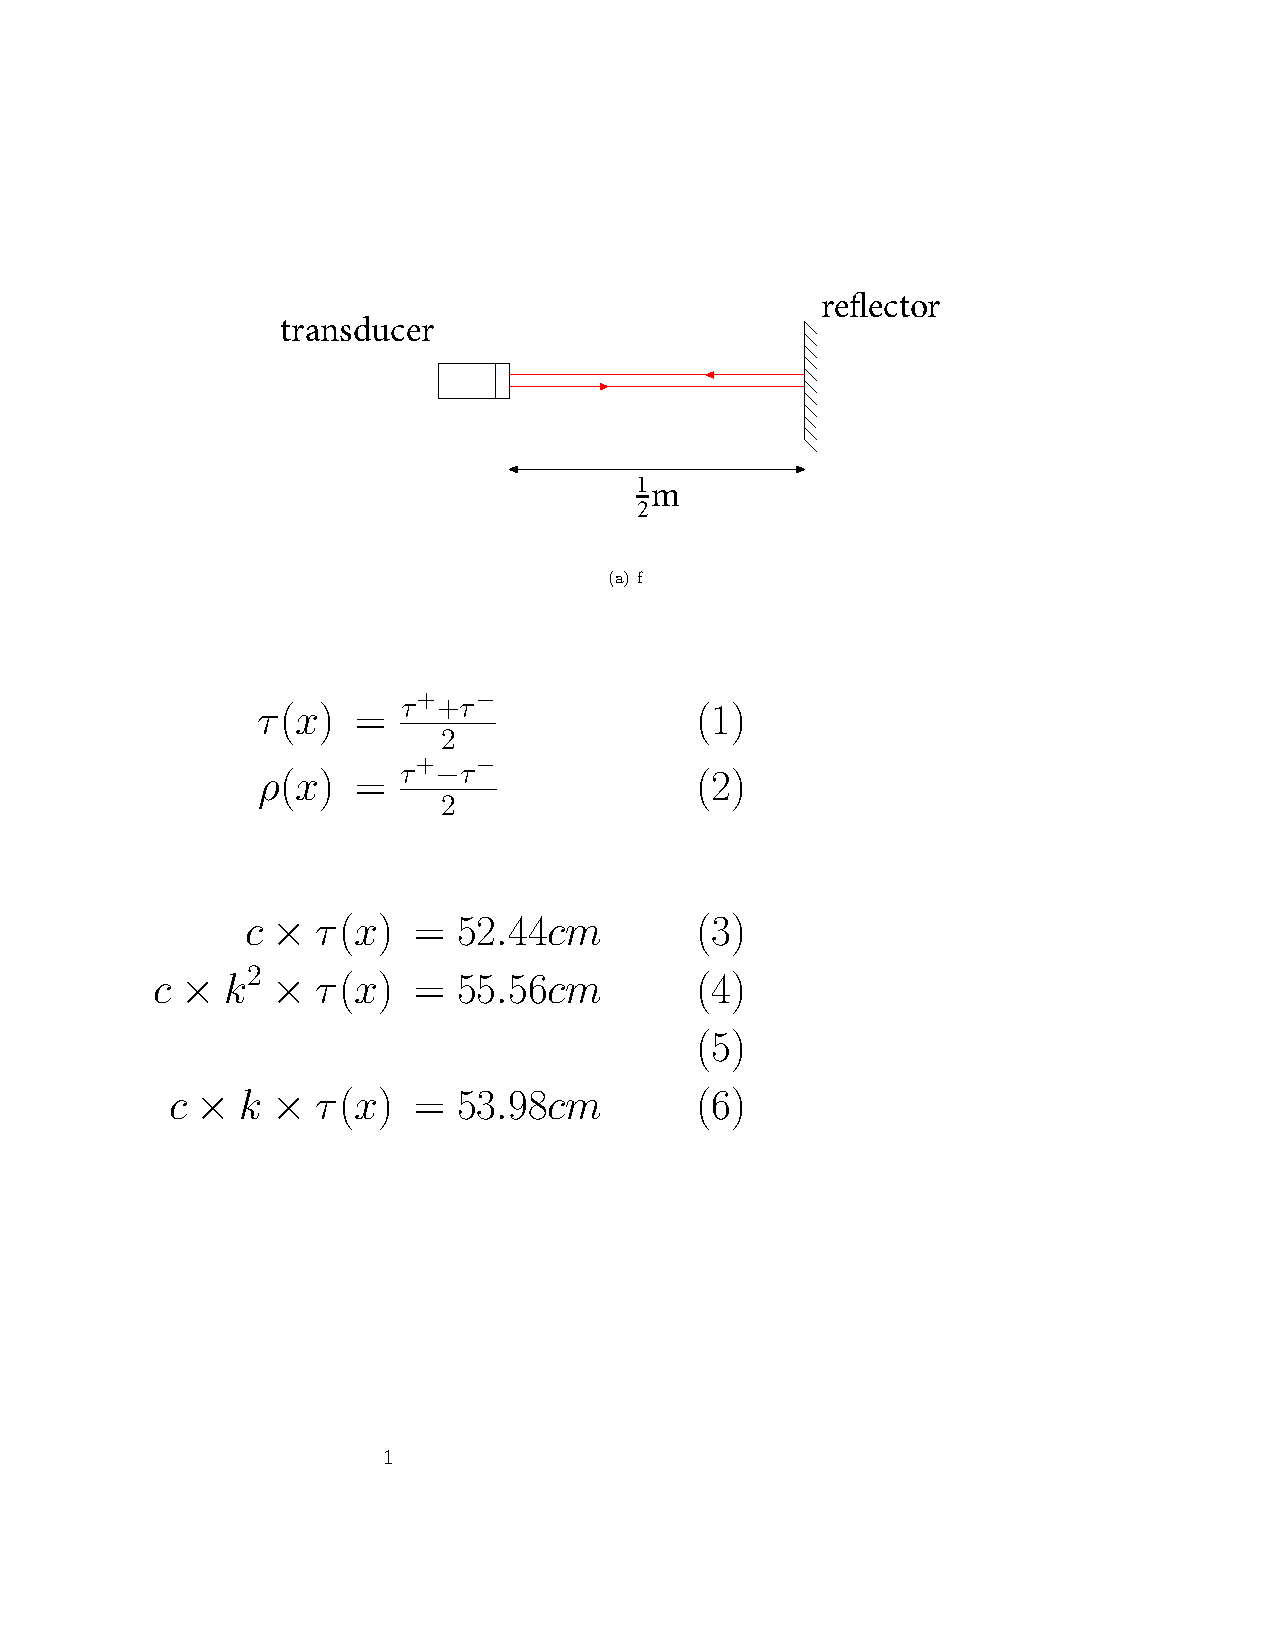
\includegraphics{measurement_figs_big2.0}}
\end{figure}

\begin{figure}%[htp]
     \centering
     \subfigure[f]{
          \label{fig:ellipse_a}
          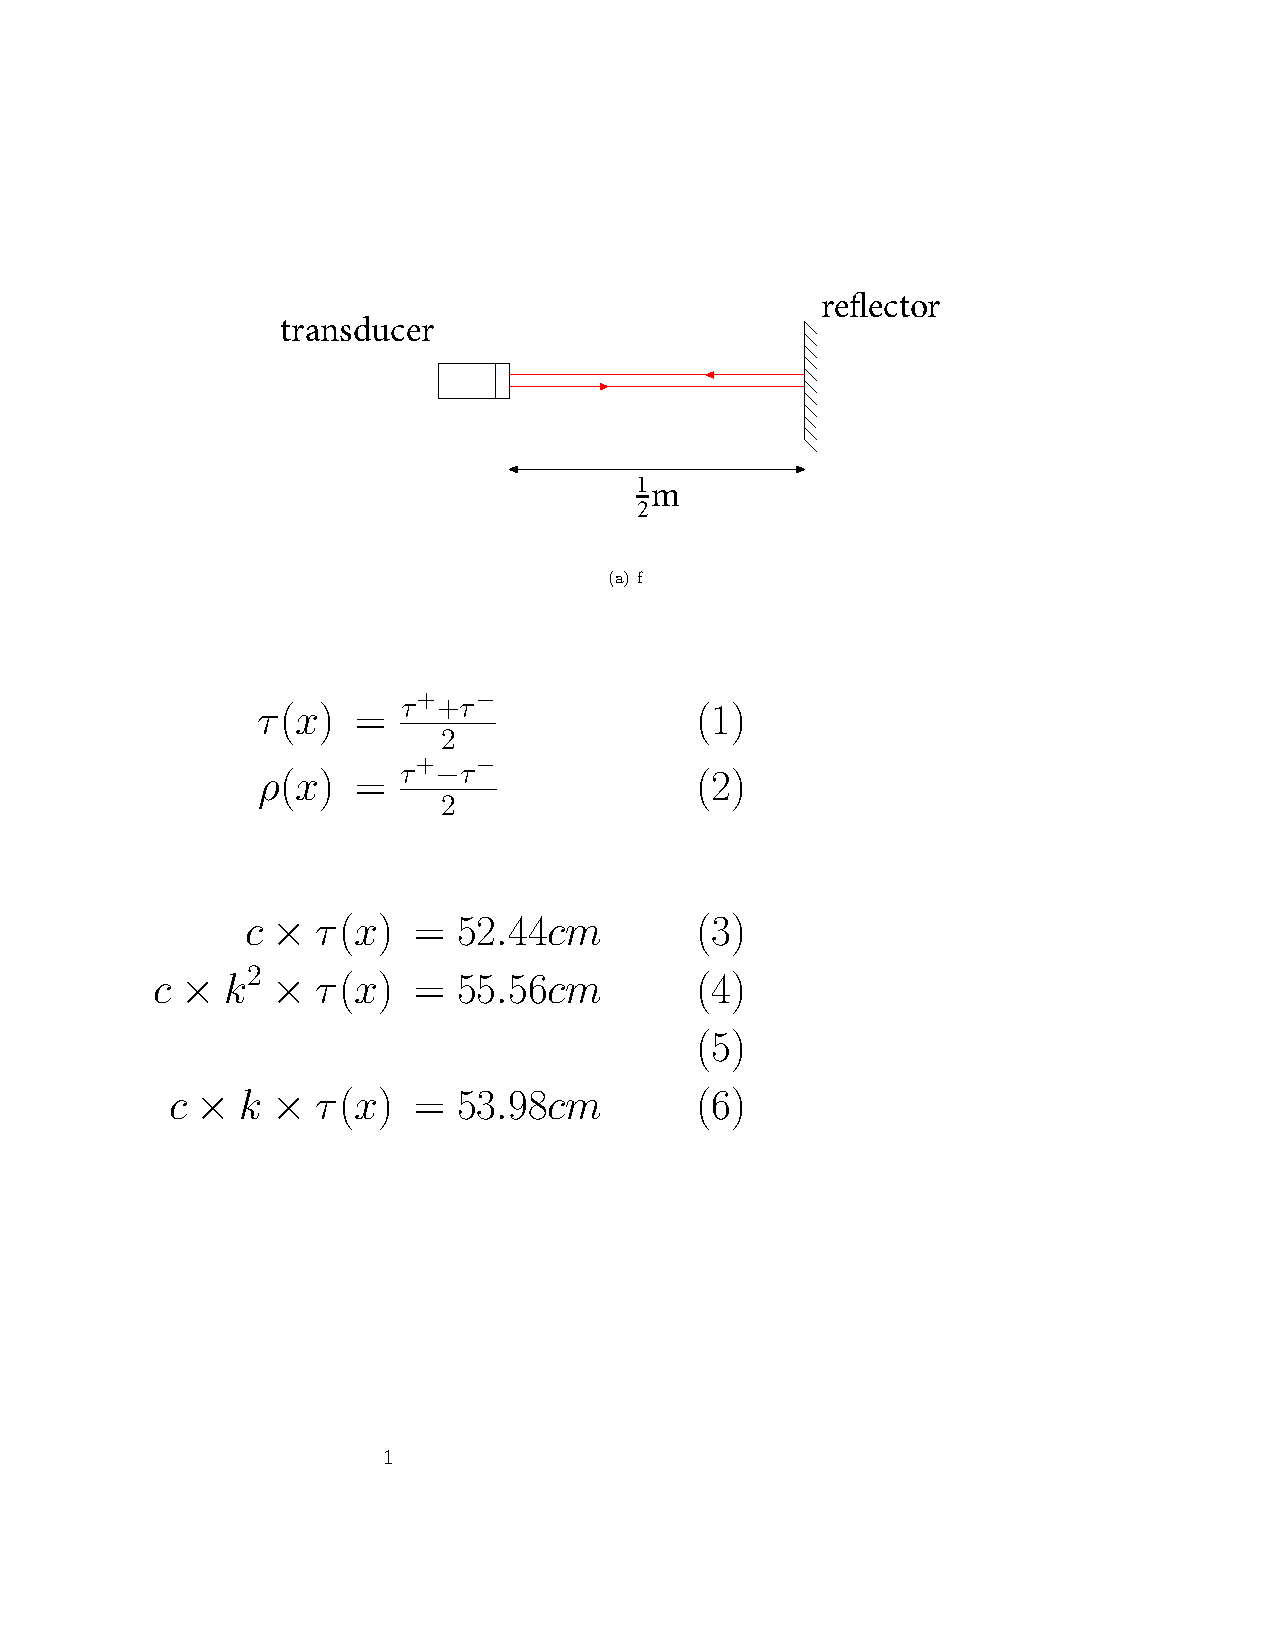
\includegraphics{measurement_figs_big2.1}}
\end{figure}


\begin{figure}%[htp]
     \centering
     \subfigure[f]{
          \label{fig:ellipse_a}
          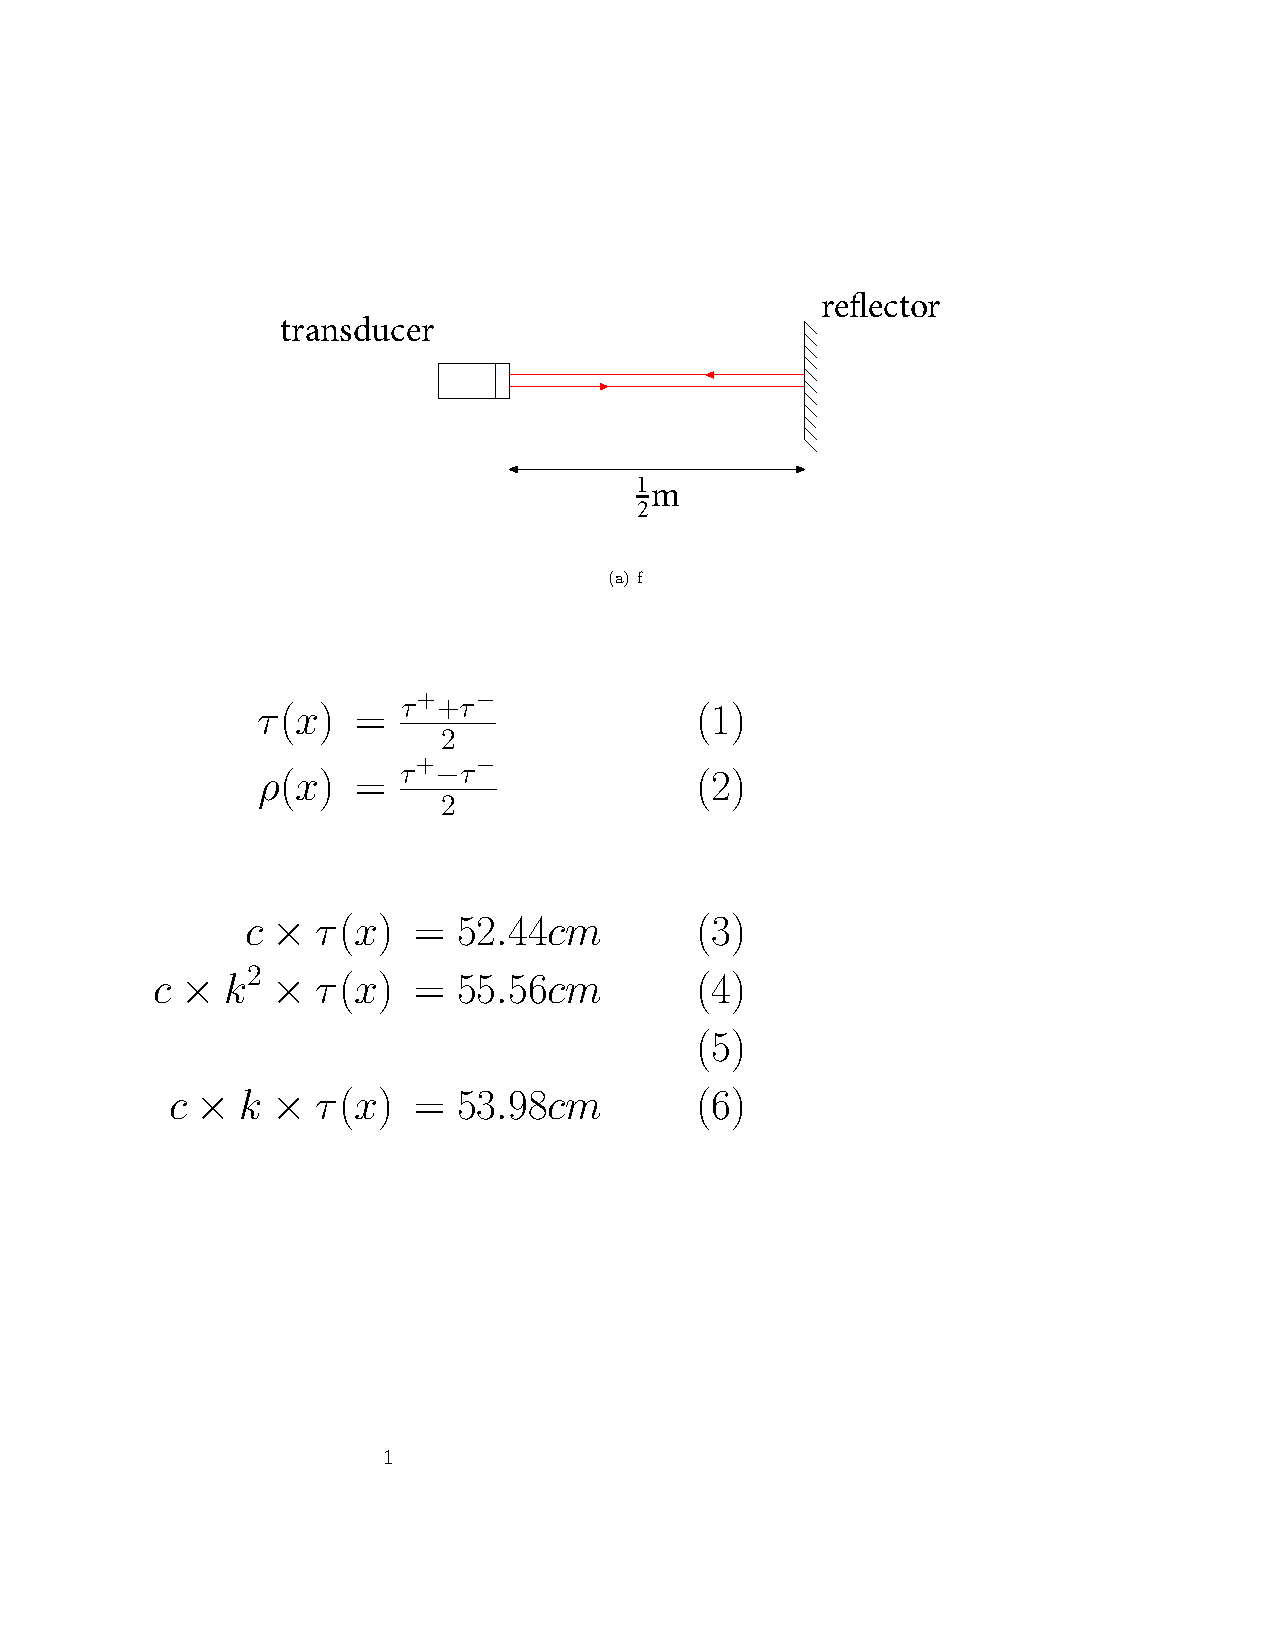
\includegraphics{measurement_figs_big2.2}}
\end{figure}


\begin{figure}%[htp]
     \centering
     \subfigure[f]{
          \label{fig:ellipse_a}
          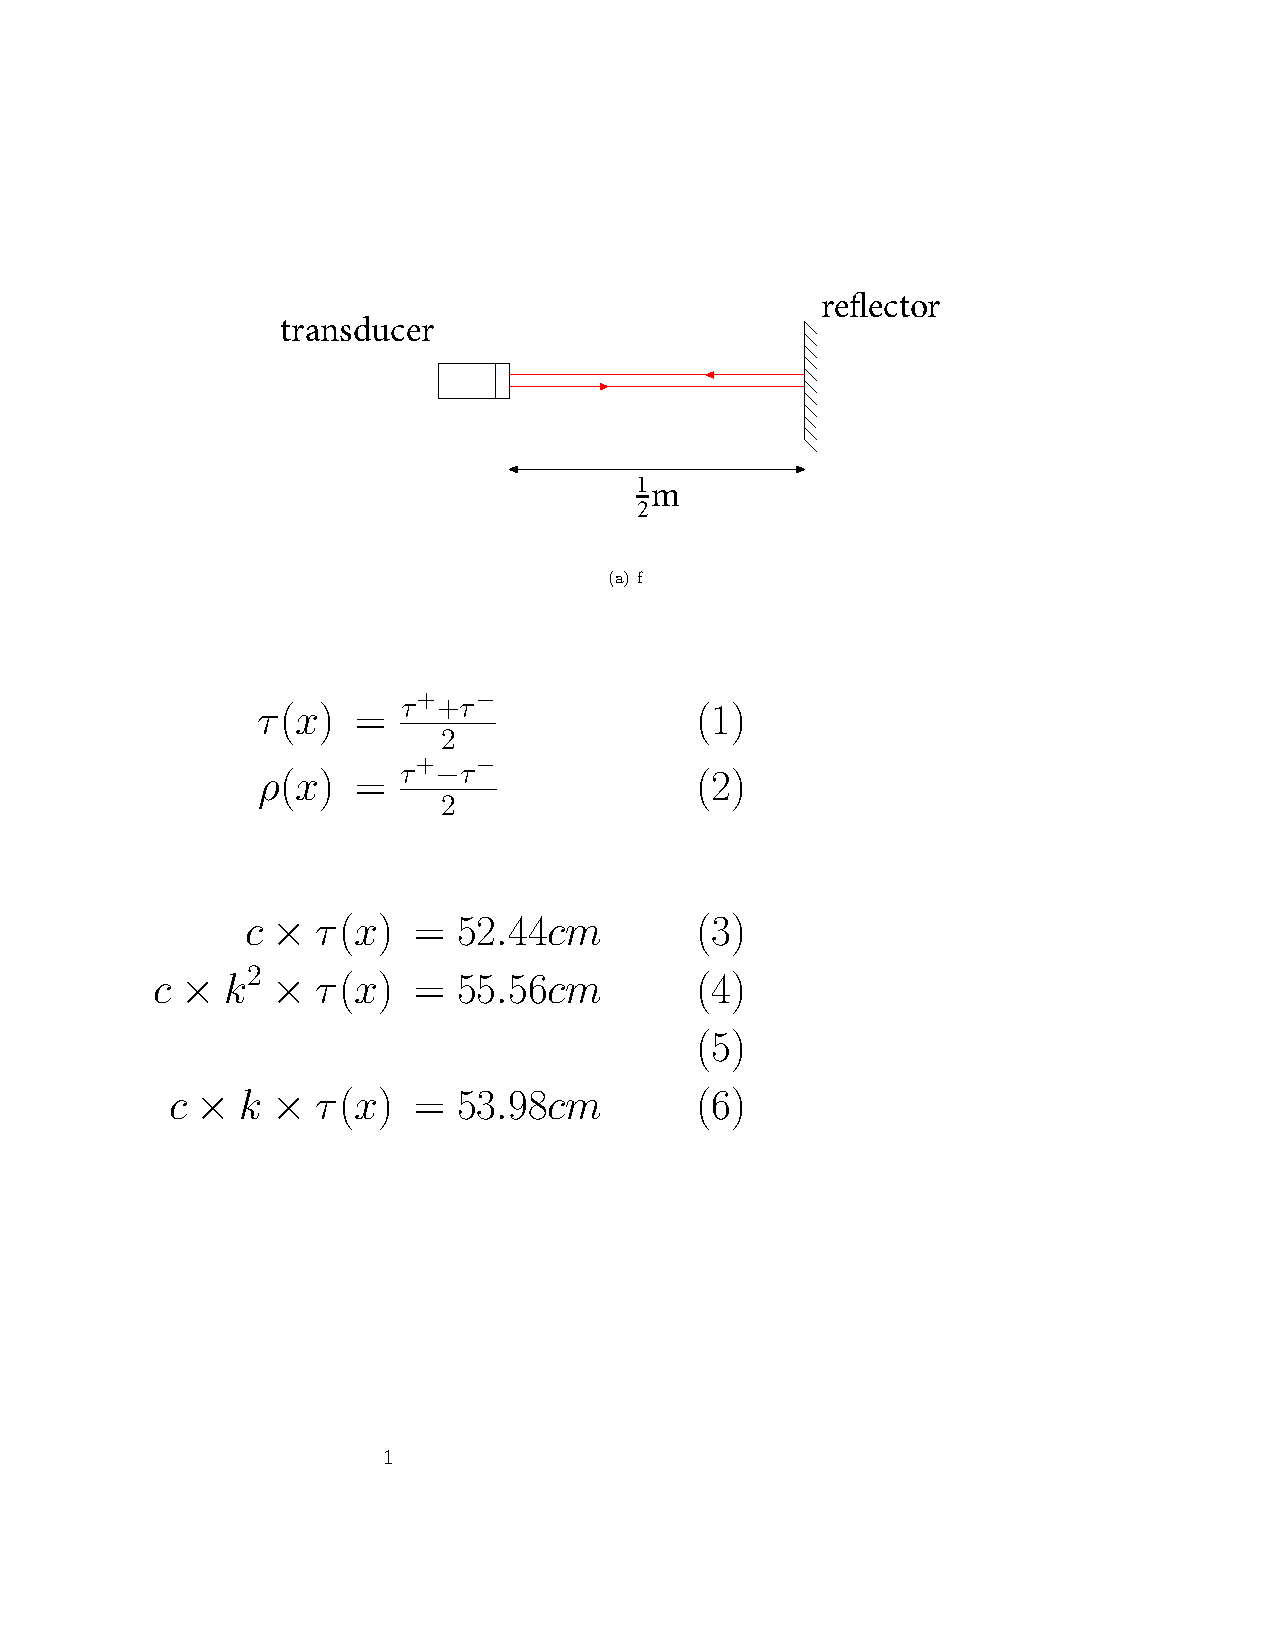
\includegraphics{measurement_figs_big2.3}}
\end{figure}


\begin{figure}%[htp]
     \centering
     \subfigure[f]{
          \label{fig:ellipse_a}
          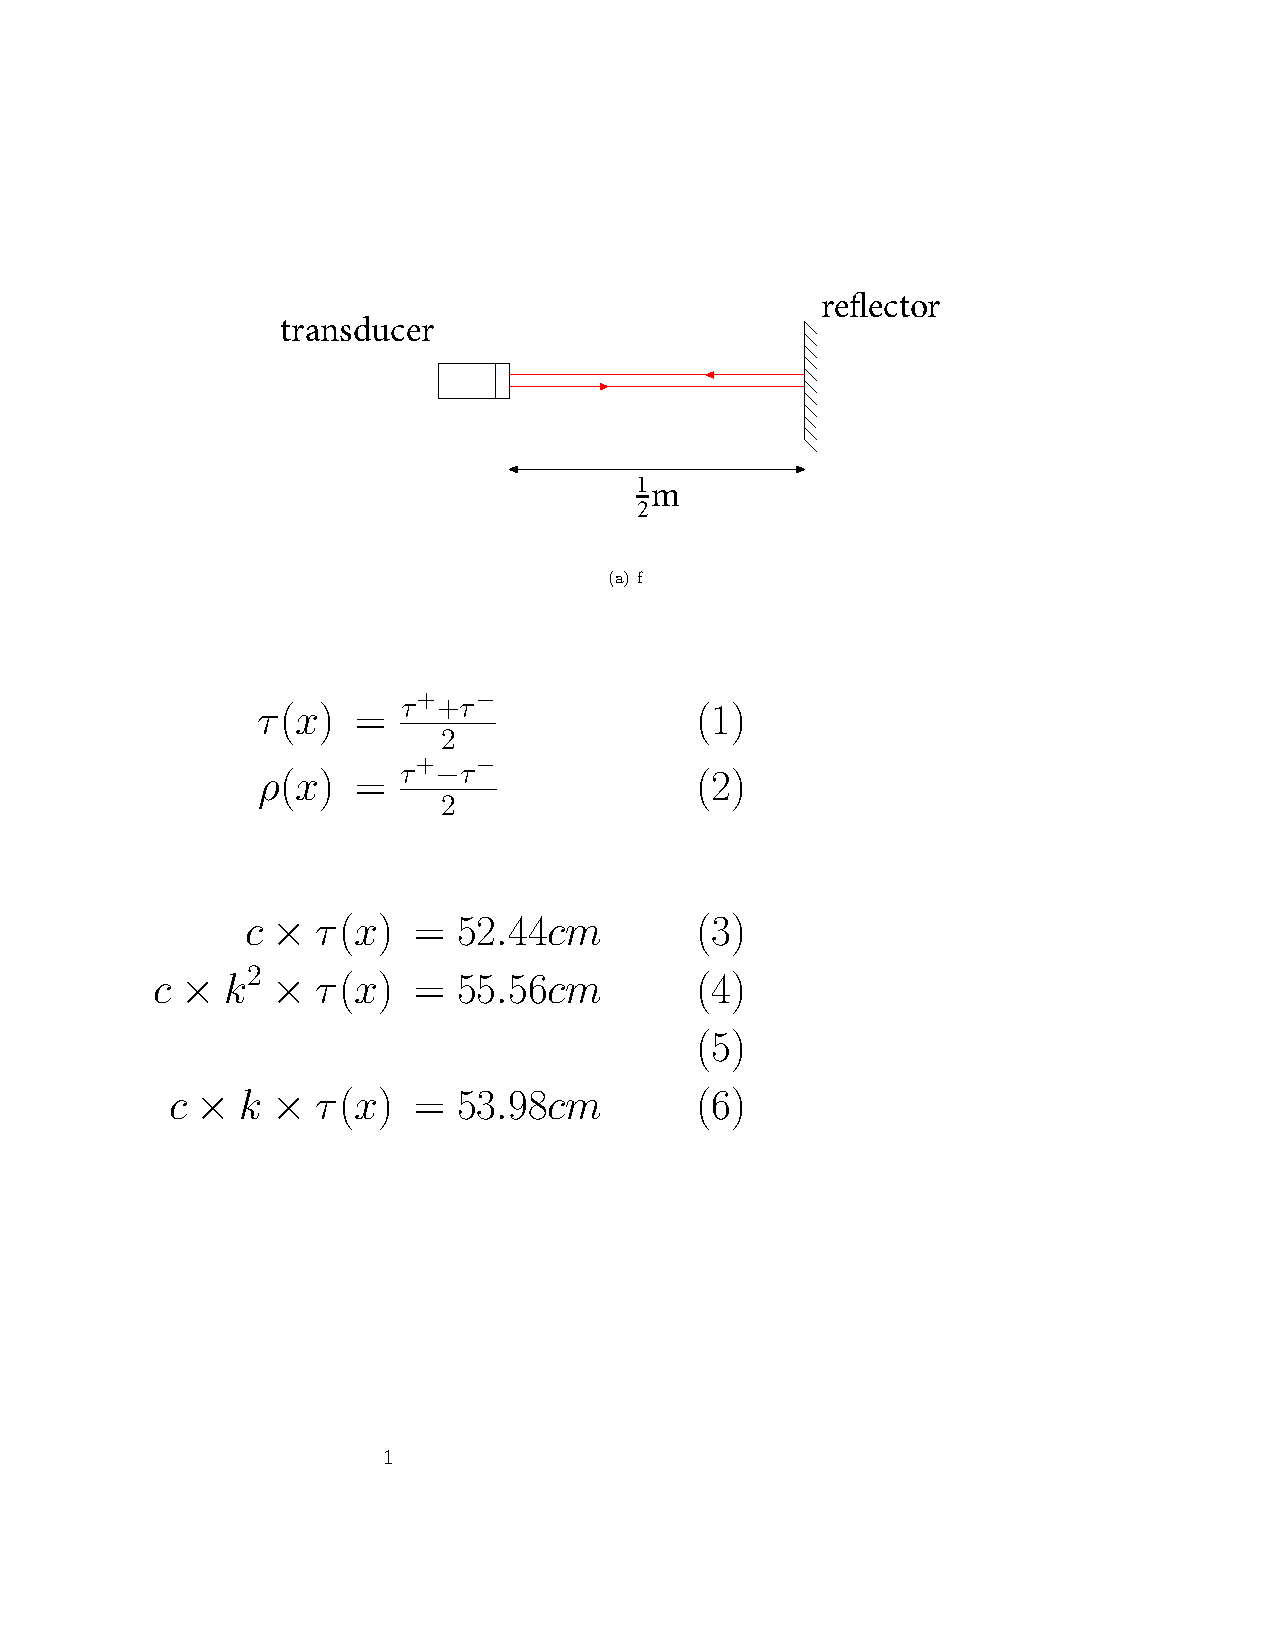
\includegraphics{measurement_figs_big2.4}}
\end{figure}


\begin{figure}%[htp]
     \centering
     \subfigure[f]{
          \label{fig:ellipse_a}
          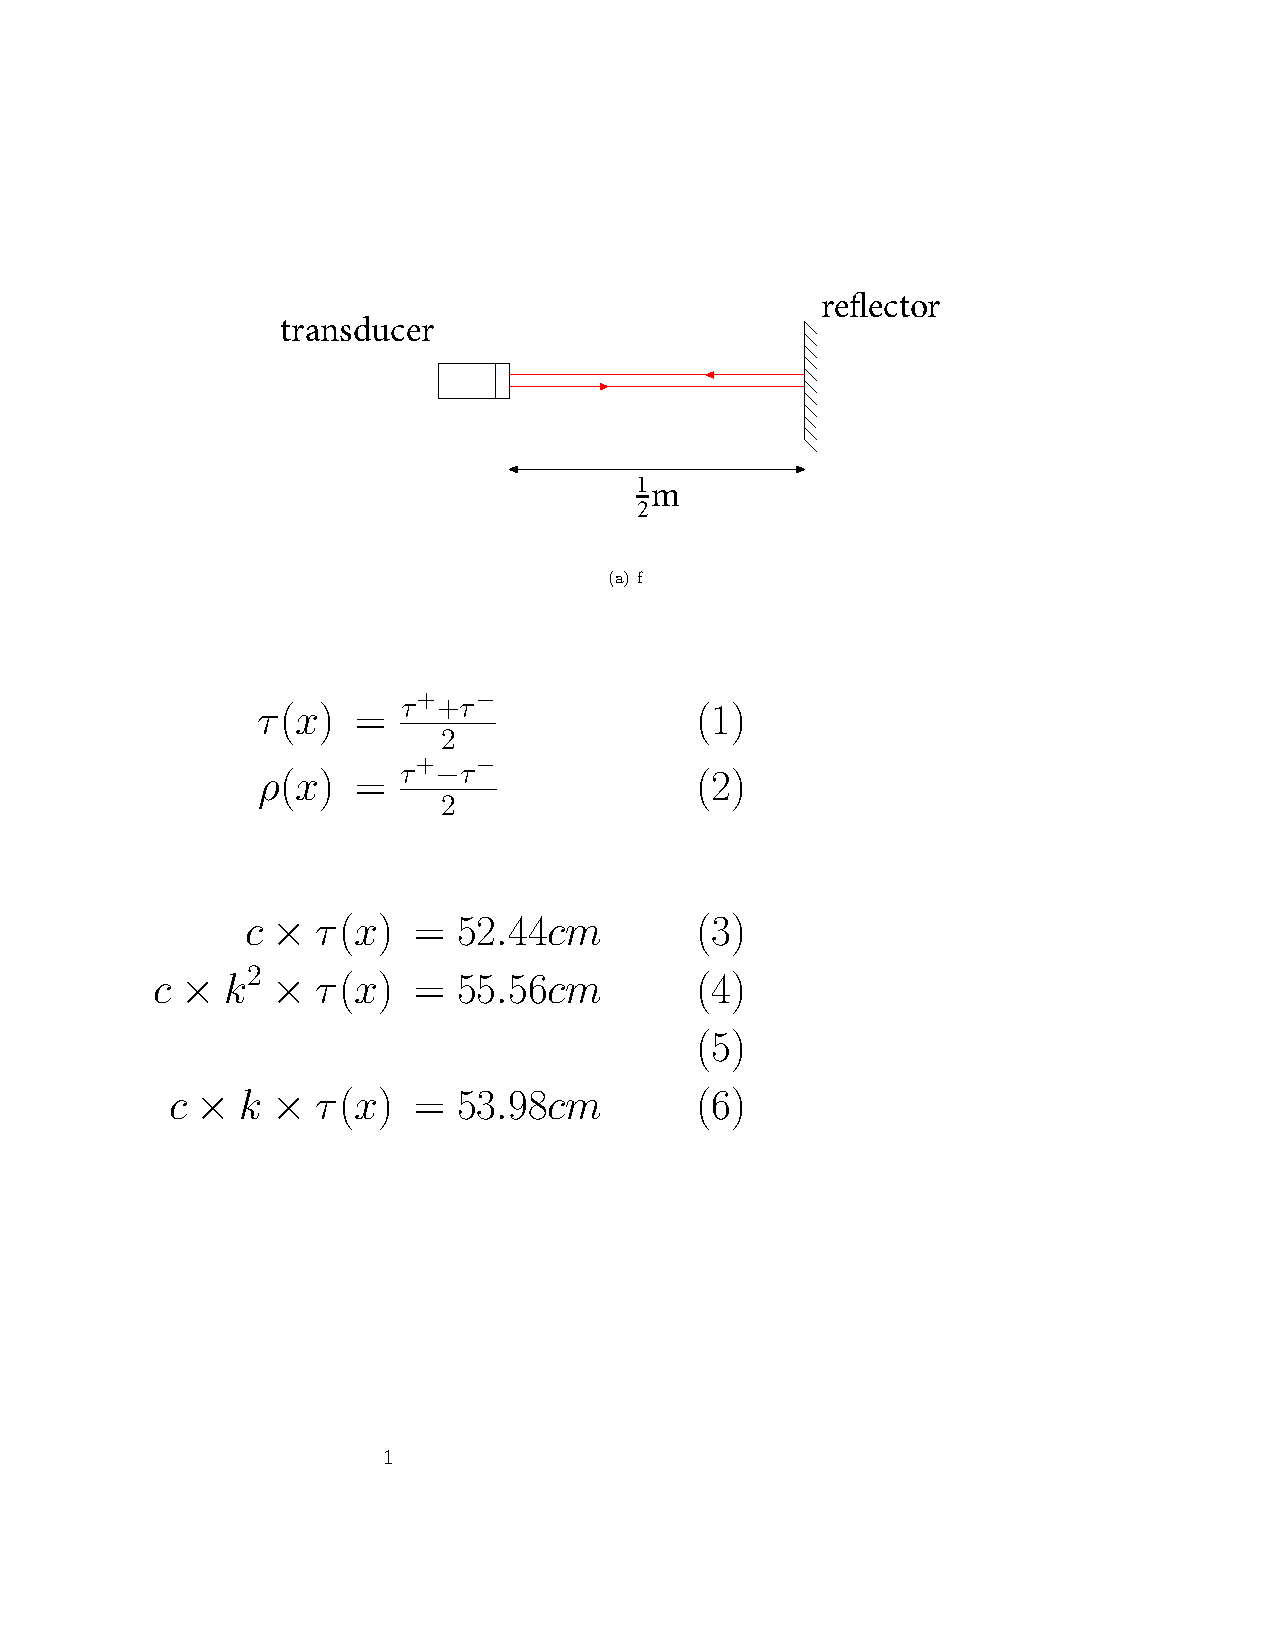
\includegraphics{measurement_figs_big2.5}}
\end{figure}


\begin{figure}%[htp]
     \centering
     \subfigure[f]{
          \label{fig:ellipse_a}
          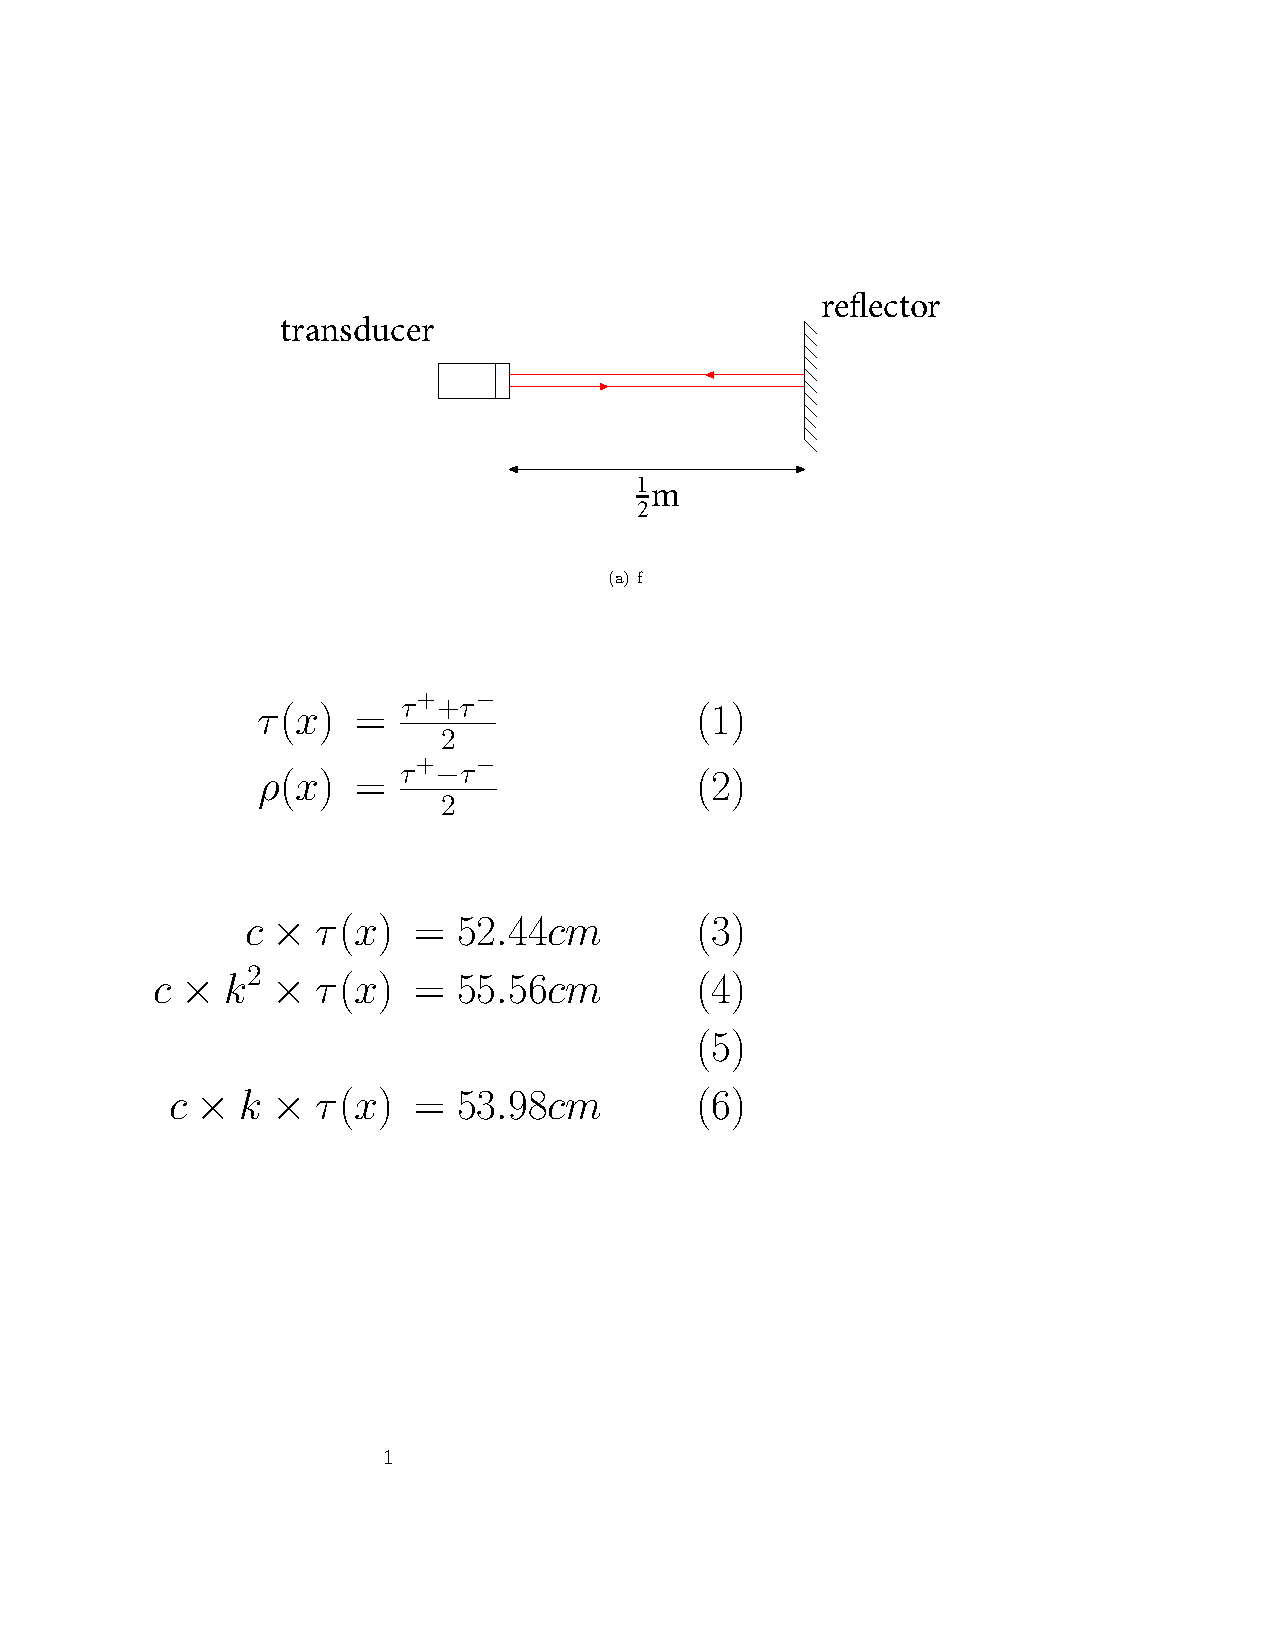
\includegraphics{measurement_figs_big2.6}}
\end{figure}


\begin{figure}%[htp]
     \centering
     \subfigure[f]{
          \label{fig:ellipse_a}
          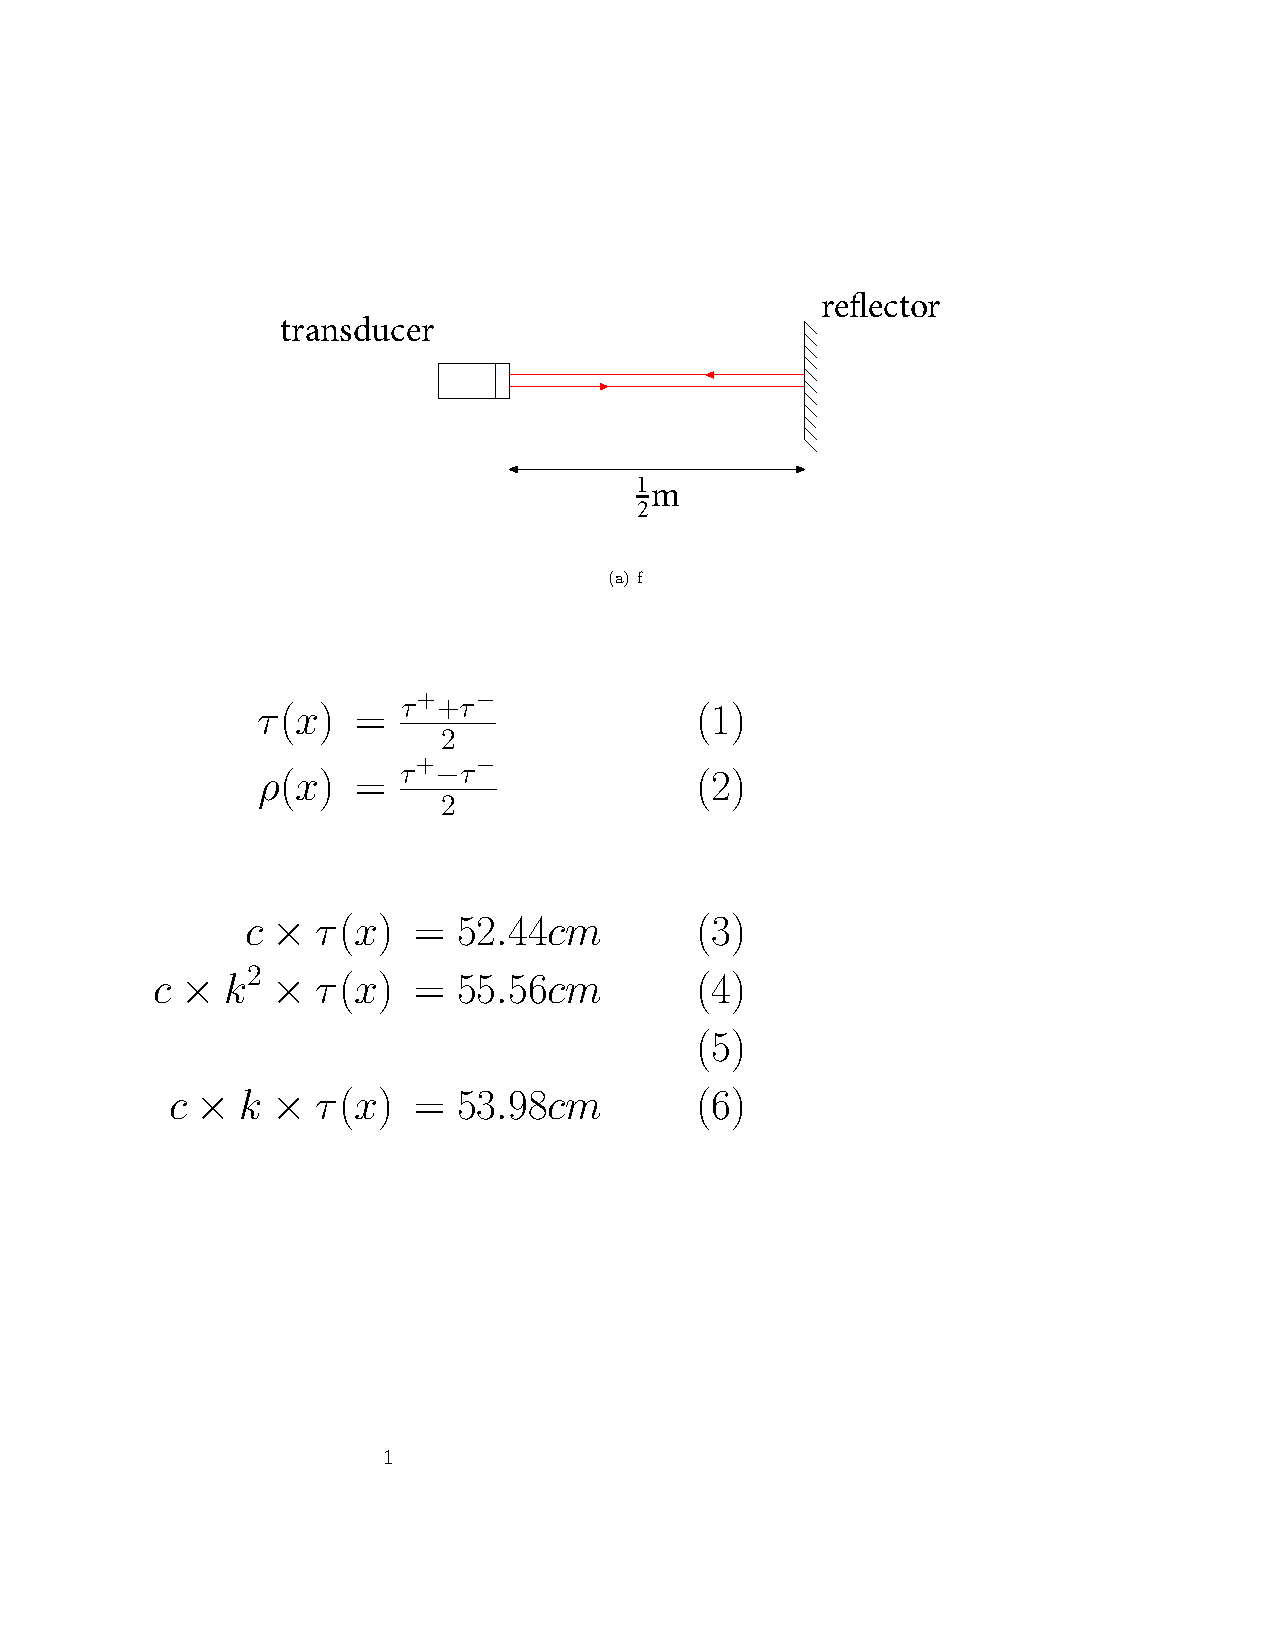
\includegraphics{measurement_figs_big2.7}}
\end{figure}




% \begin{figure}%[htp]
%      \centering
%      \subfigure[f]{
%           \label{fig:ellipse_a}
%           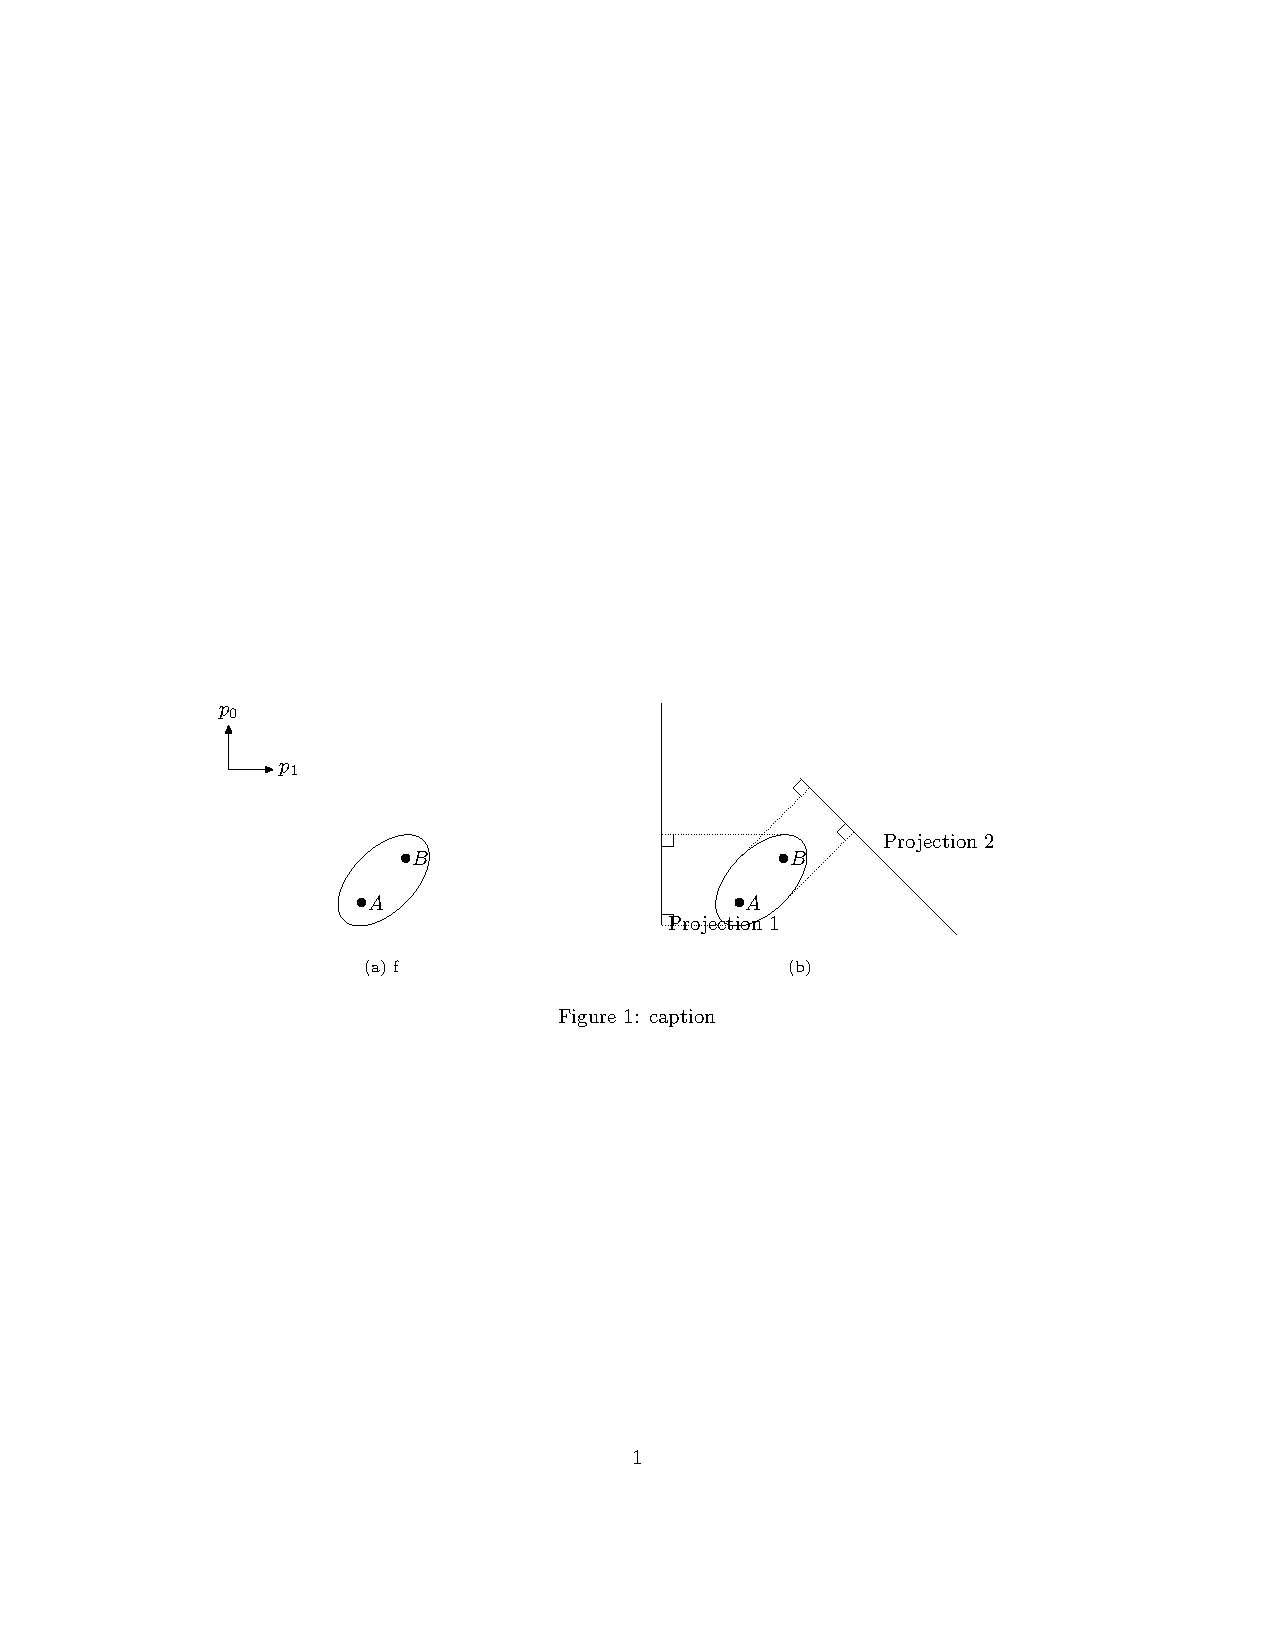
\includegraphics{measurement.2}}
%      \hspace{3cm}
%      \subfigure[]{
%           \label{fig:ellipse_b}
%           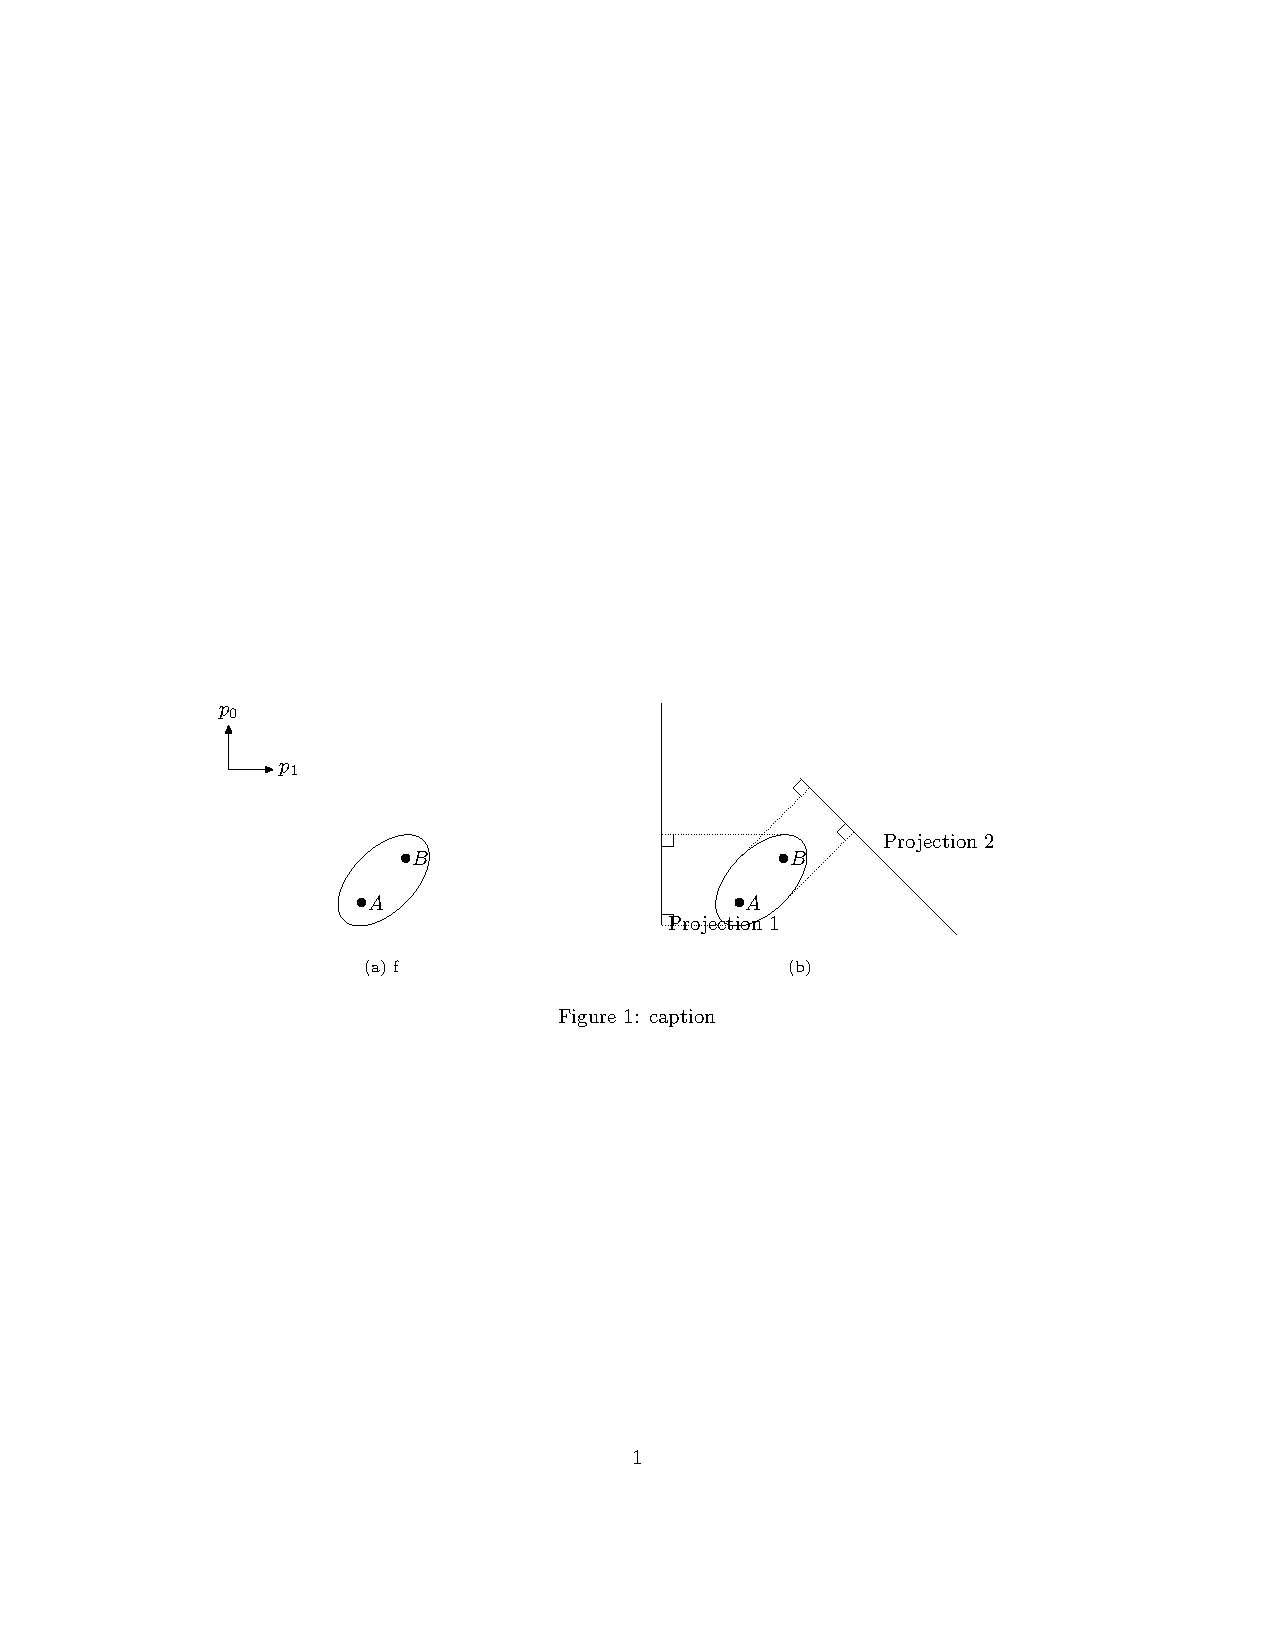
\includegraphics{measurement.11}}
    
%      \caption{caption}
%      \label{fig:ellipse}
% \end{figure}

% \begin{figure}%[htp]
%  \centering
%  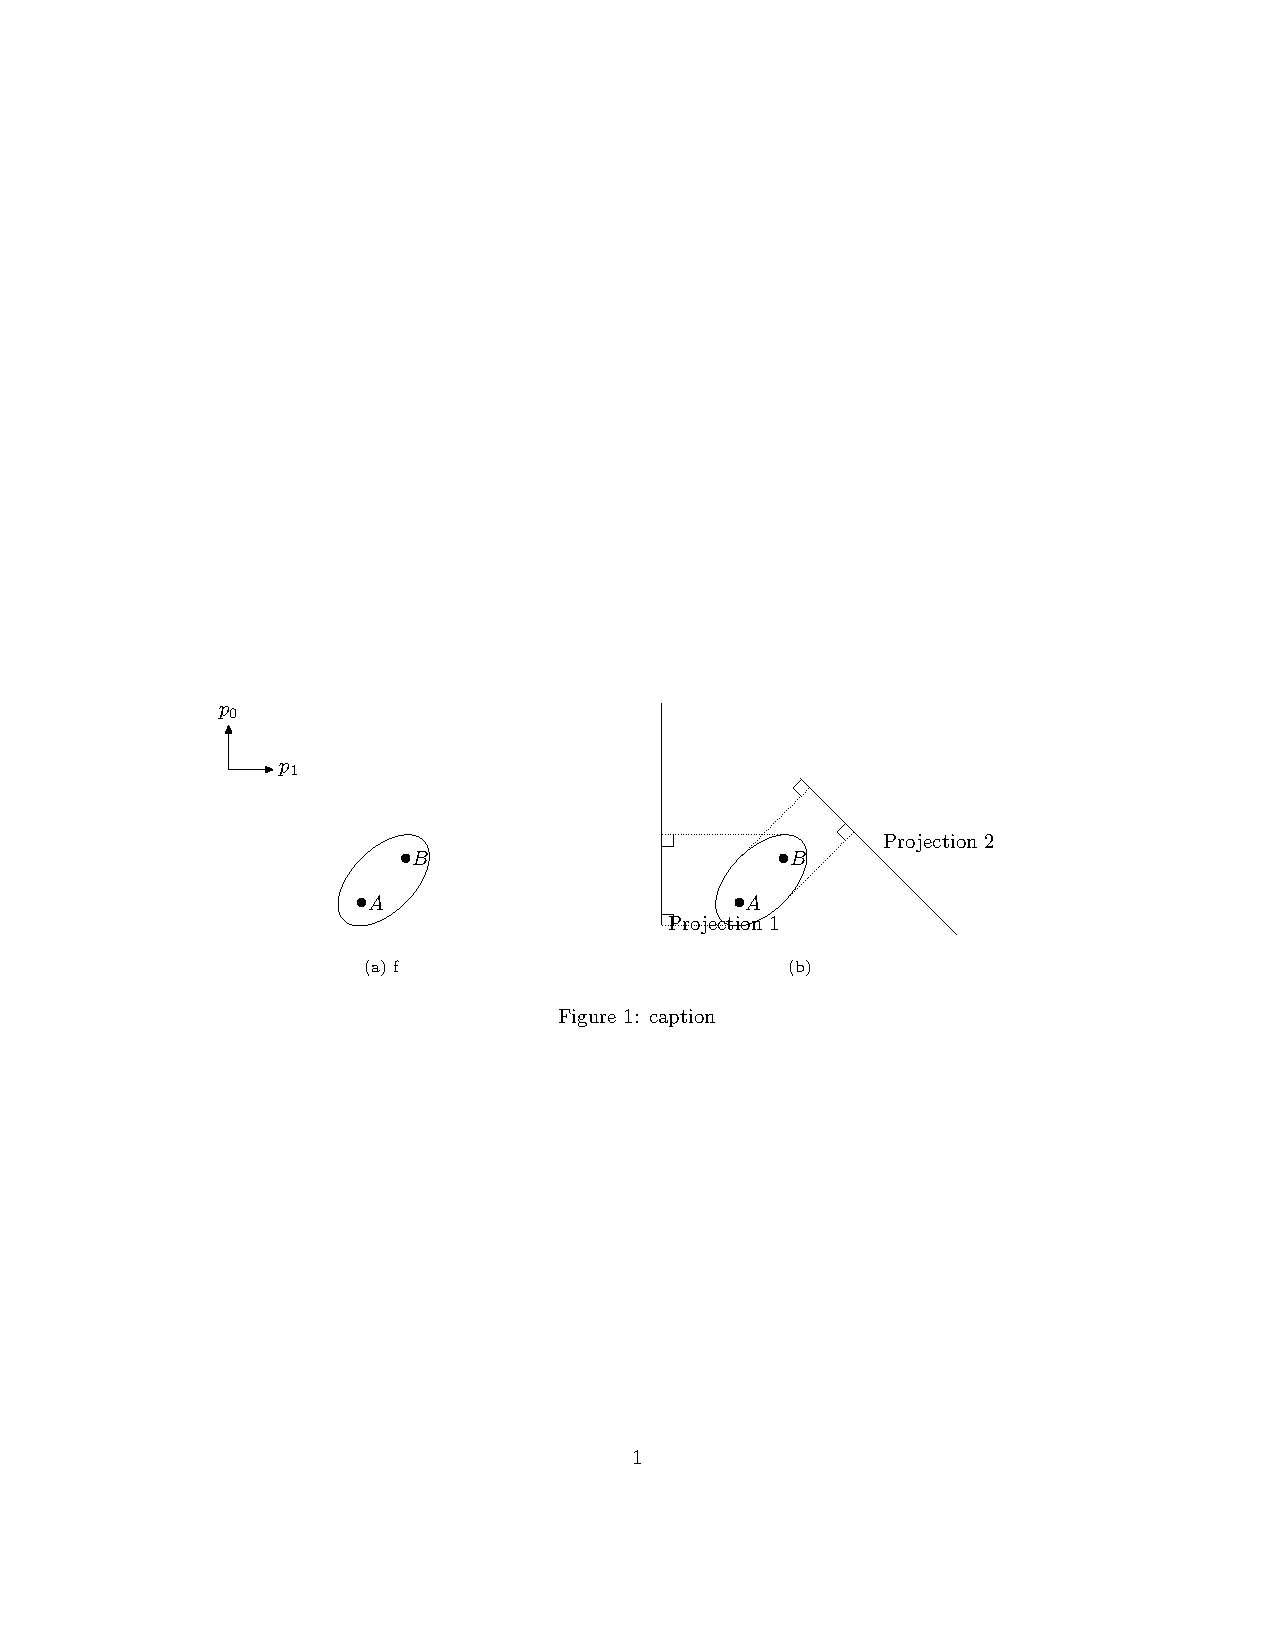
\includegraphics{measurement.2}
%  \caption{caption}
%  \label{fig:ObsEuclid}
% \end{figure}

% \begin{figure}%[htp]
%      \centering
%      \subfigure[]{
%           \label{fig:ObsA}
%           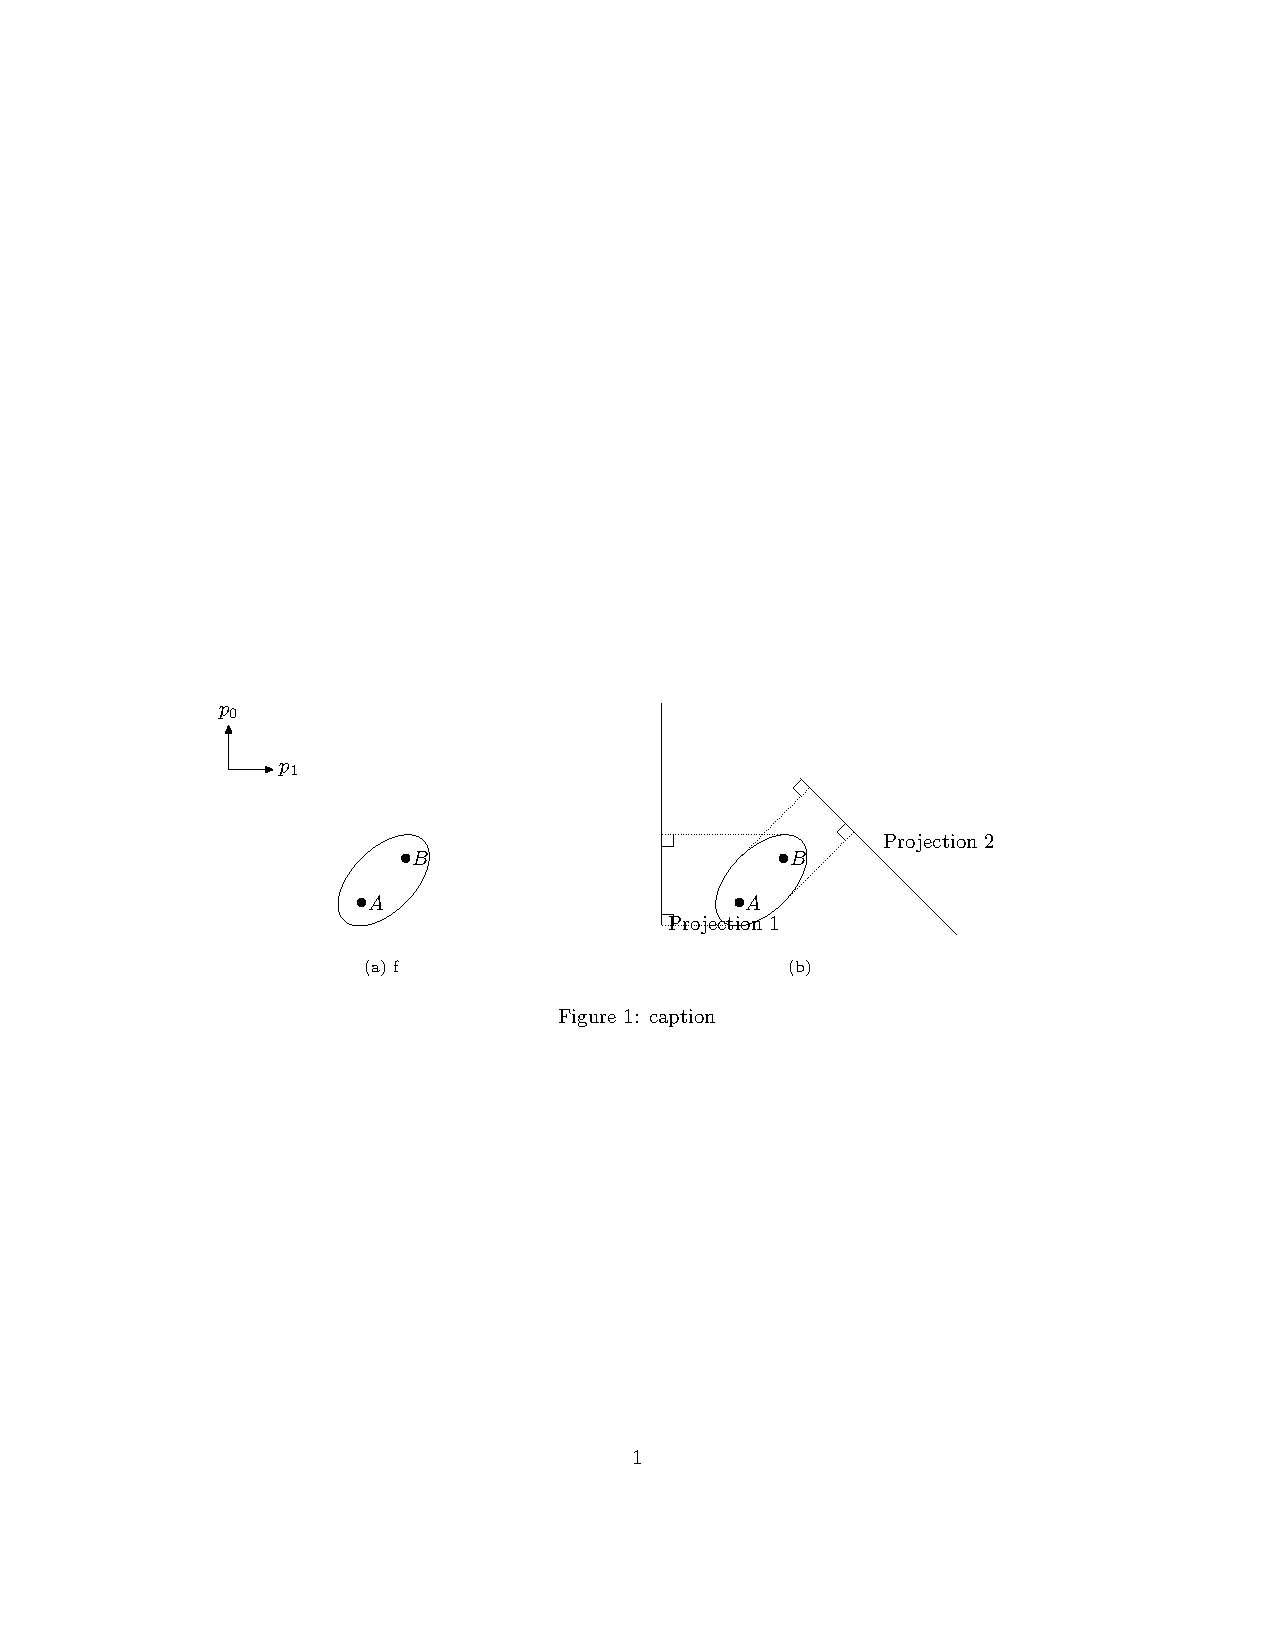
\includegraphics{measurement.3}}
%      \hspace{1cm}
%      \subfigure[]{
%           \label{fig:ObsB}
%           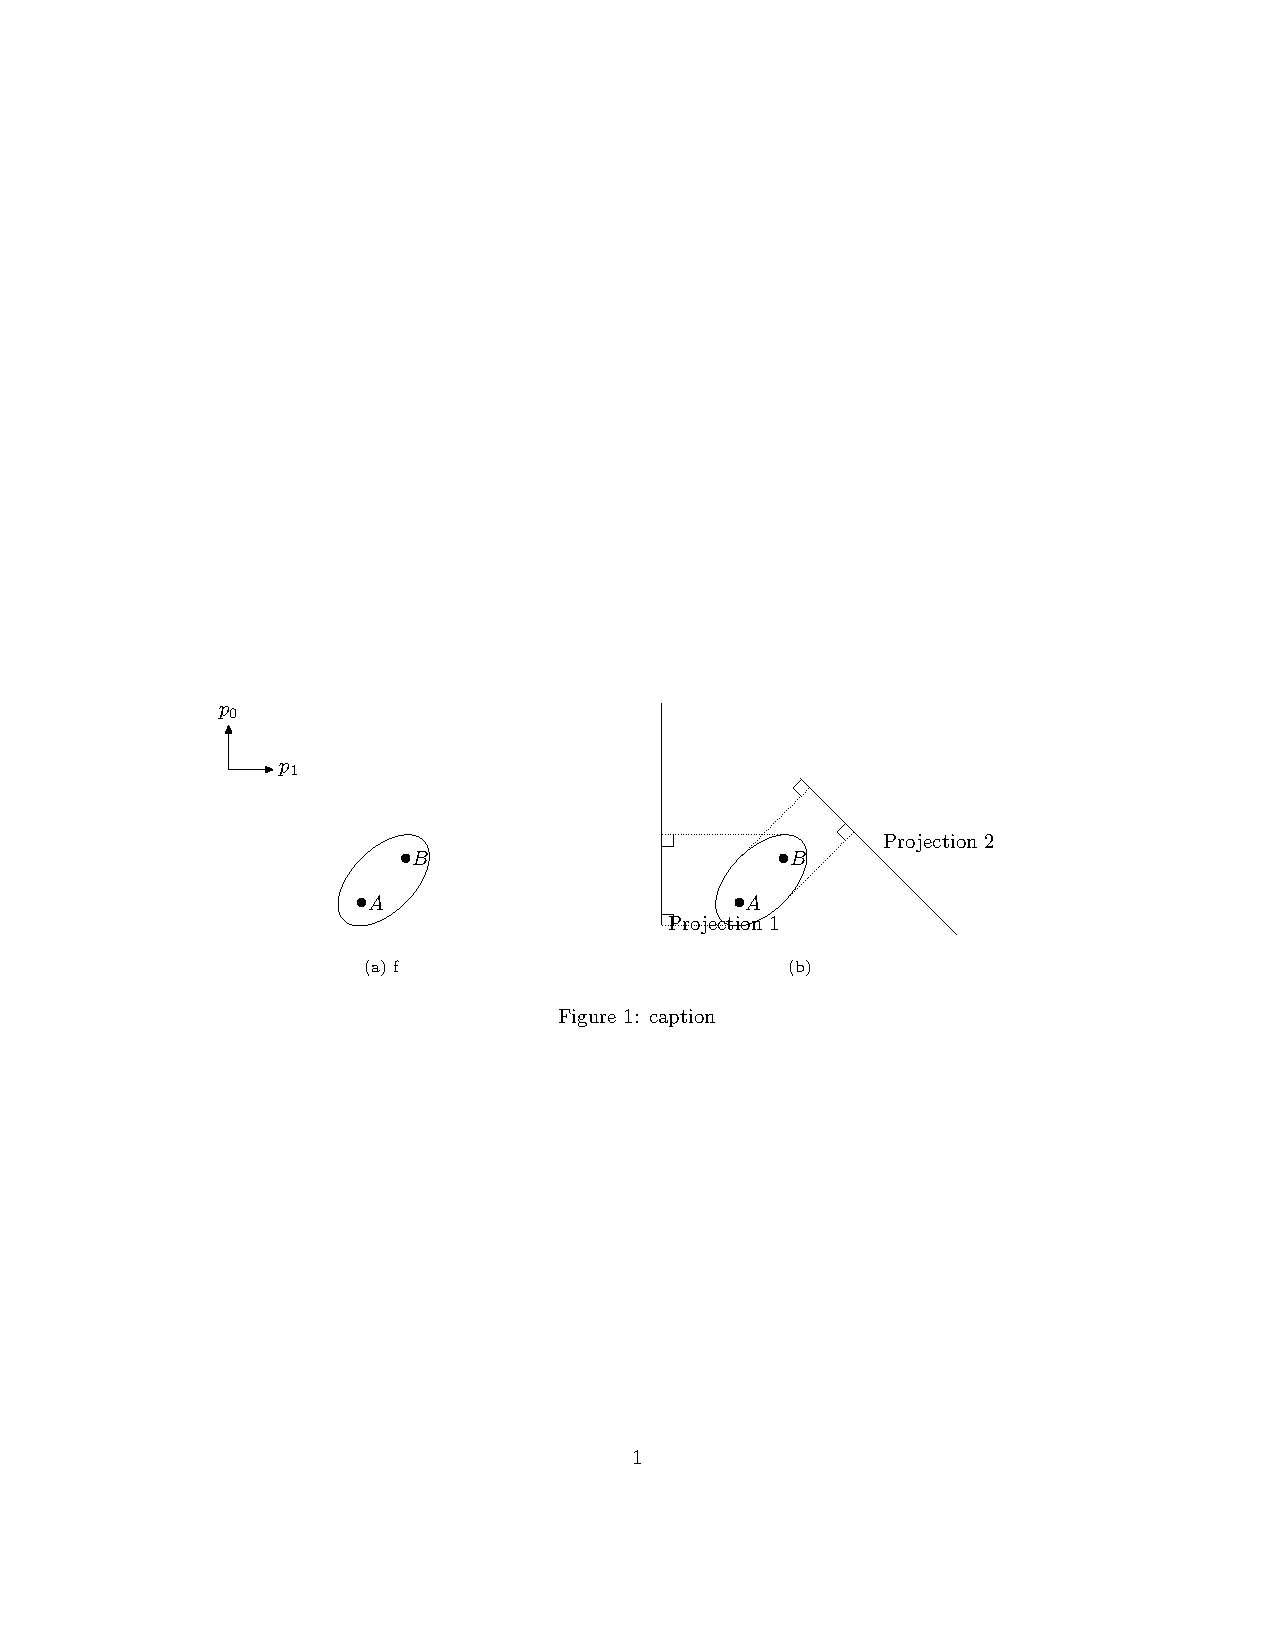
\includegraphics{measurement.4}}
%      \caption{caption}
%      \label{fig:Obs}
% \end{figure}

% \begin{figure}%[htp]
%      \centering
%      \subfigure[]{
%           \label{fig:ObsA}
%           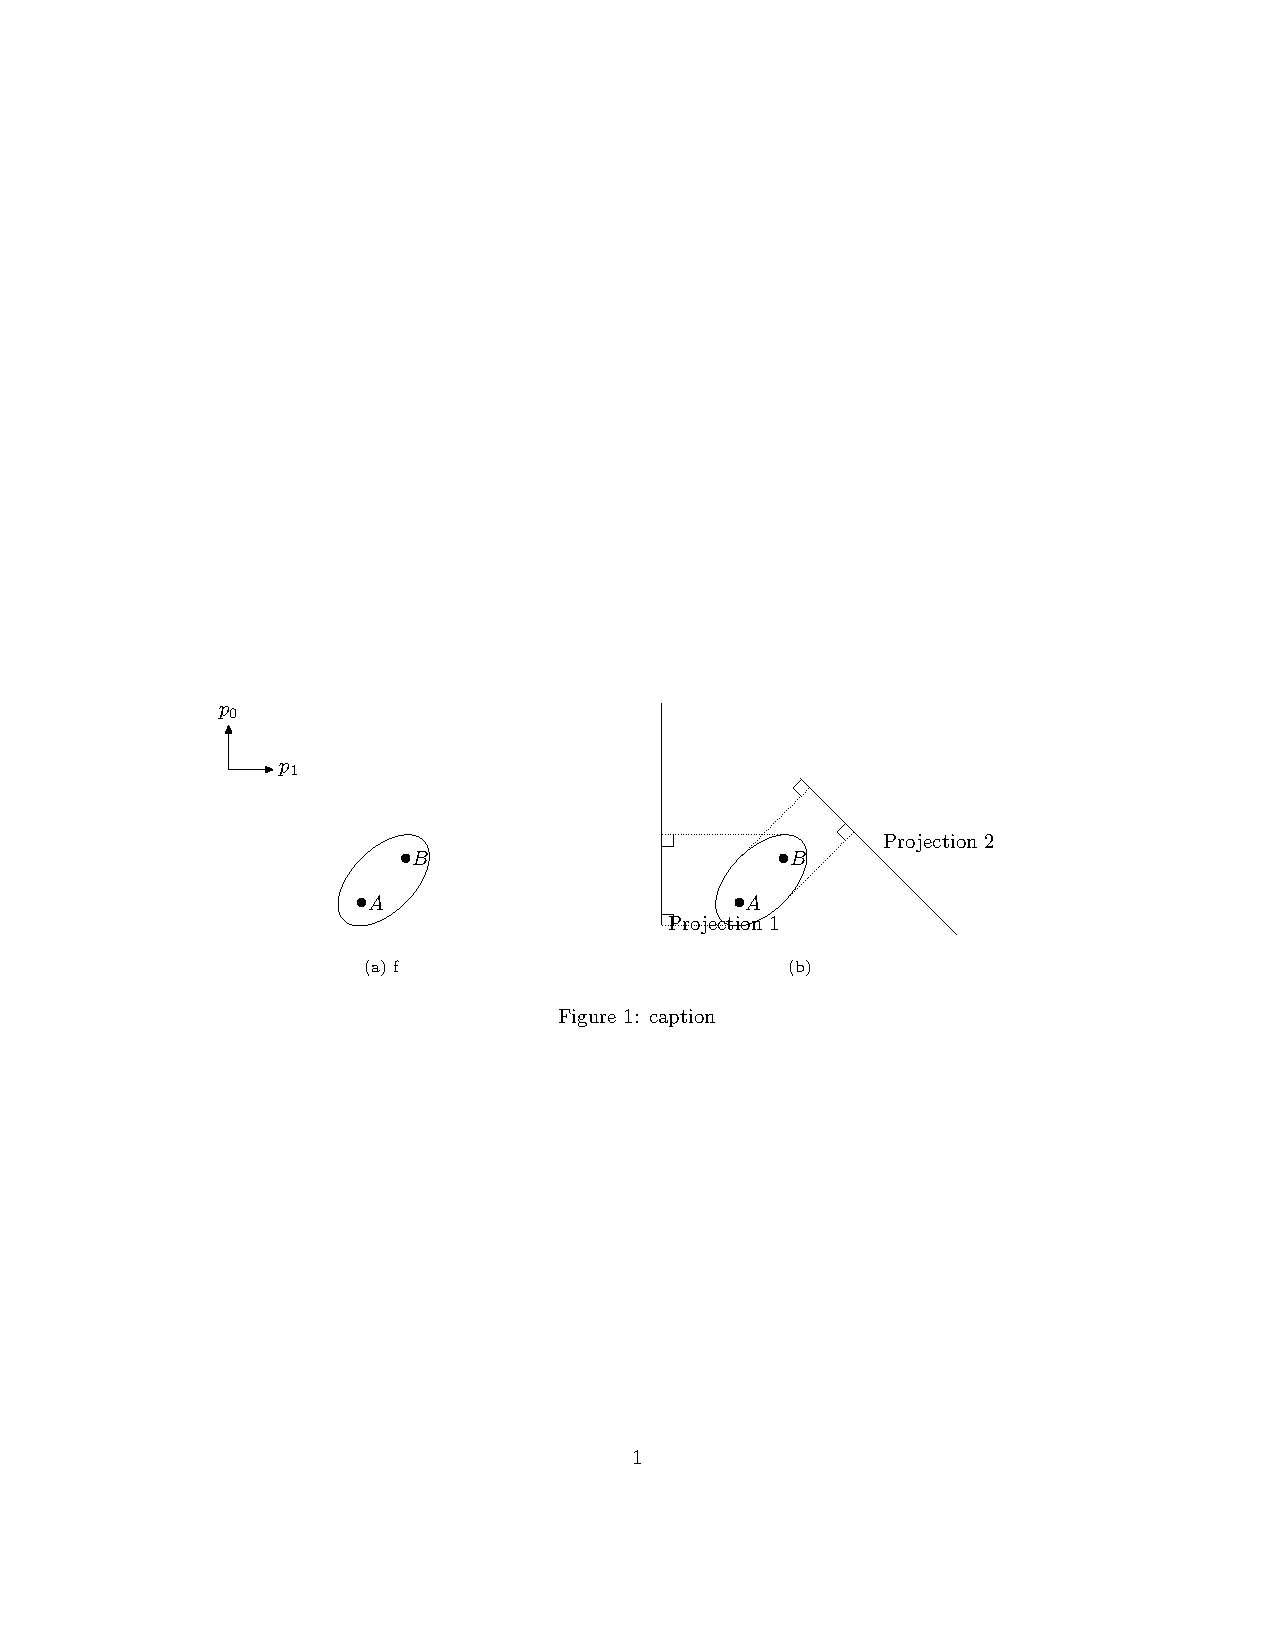
\includegraphics{measurement.5}}
%      \hspace{1cm}
%      \subfigure[]{
%           \label{fig:ObsB}
%           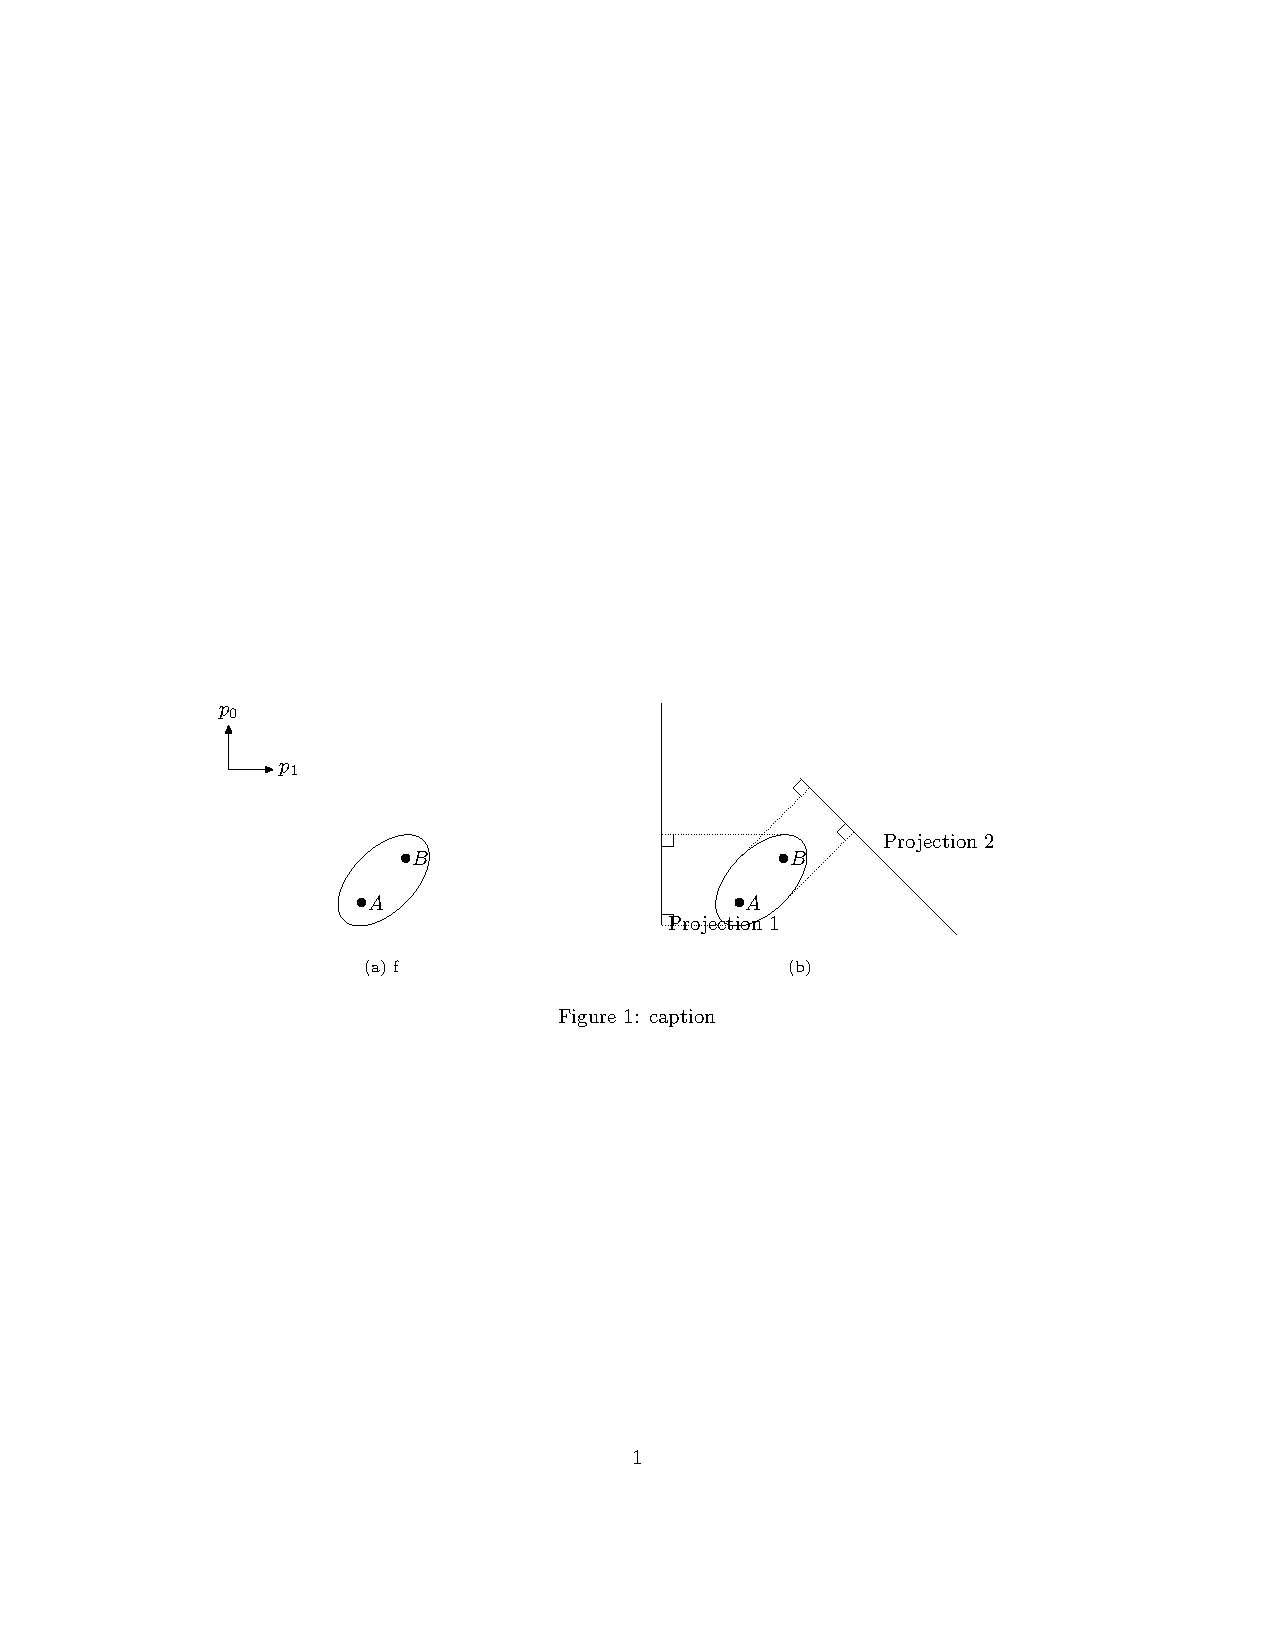
\includegraphics{measurement.6}}
%      \caption{caption}
%      \label{fig:Obs}
% \end{figure}

% \begin{figure}%[htp]
%      \centering
%      \subfigure[]{
%           \label{fig:ObsA}
%           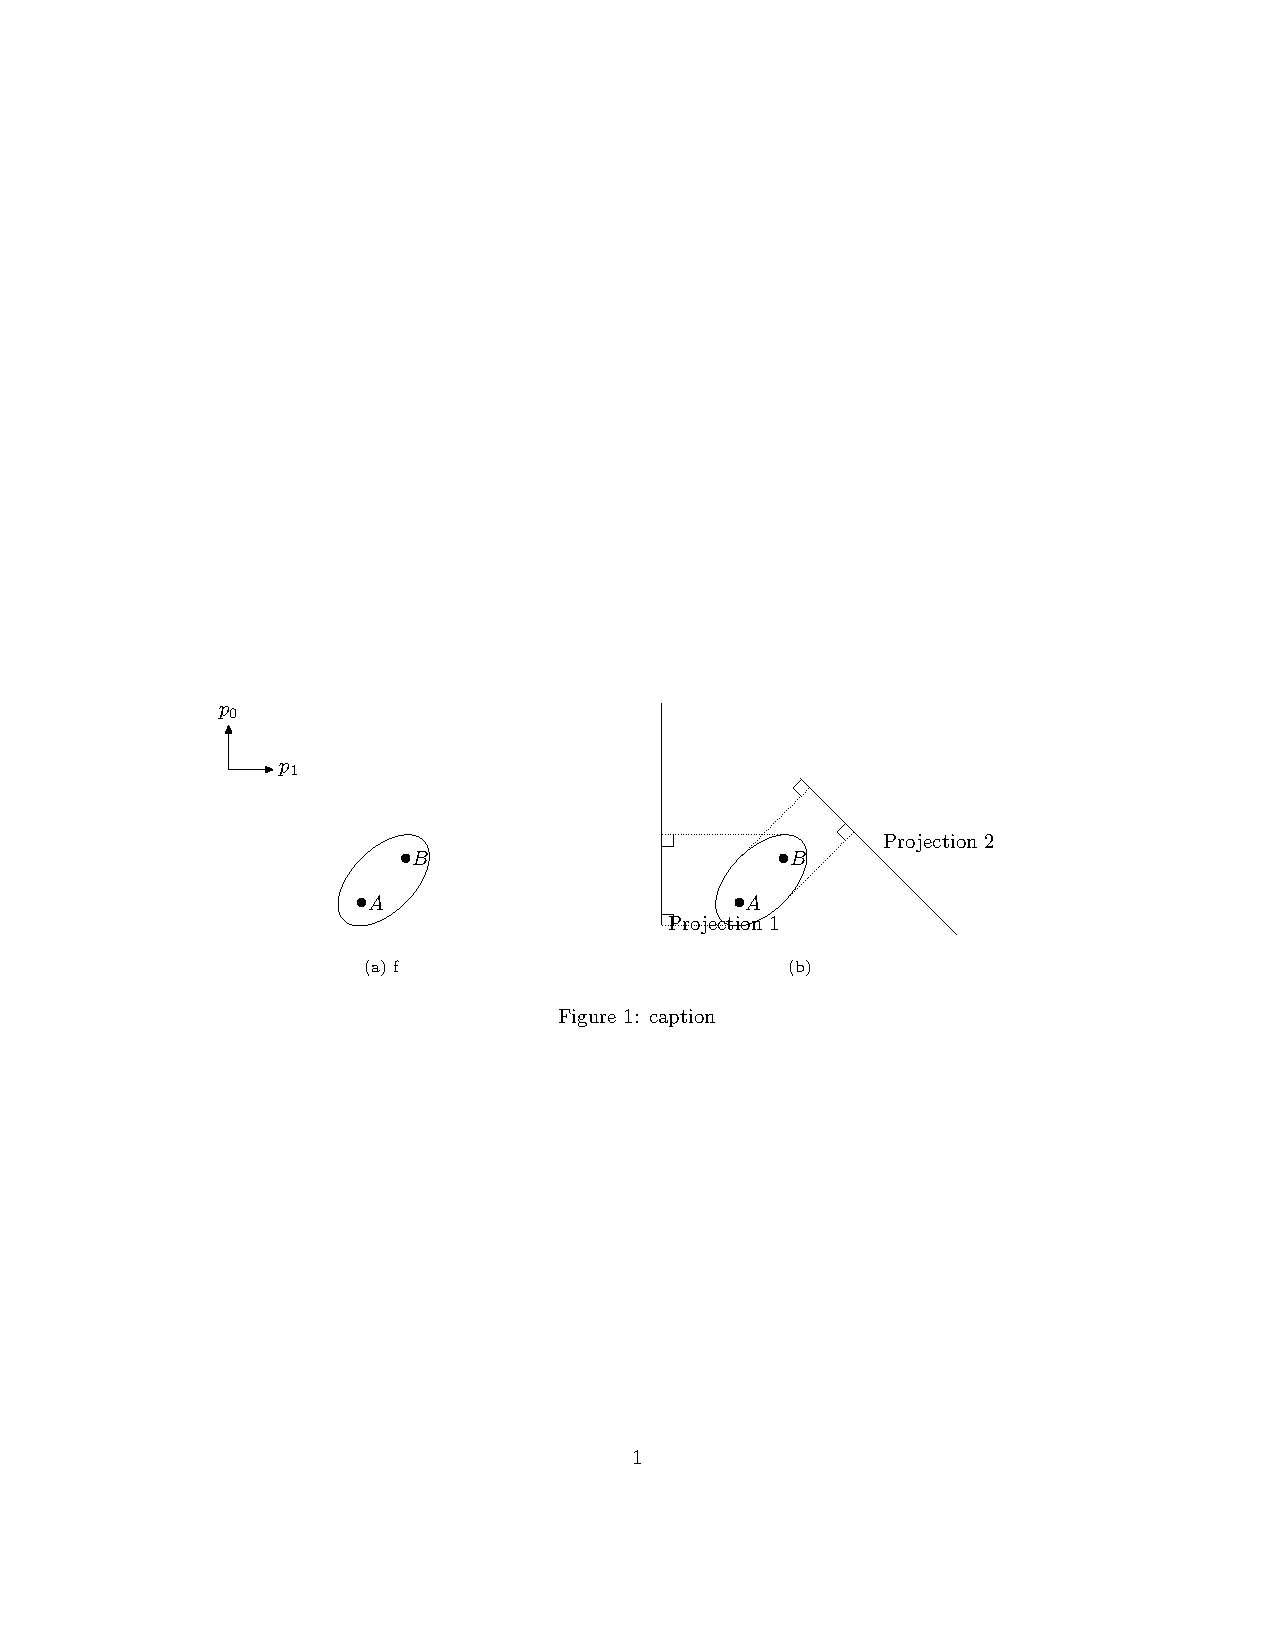
\includegraphics{measurement.7}}
%      \hspace{1cm}
%      \subfigure[]{
%           \label{fig:ObsB}
%           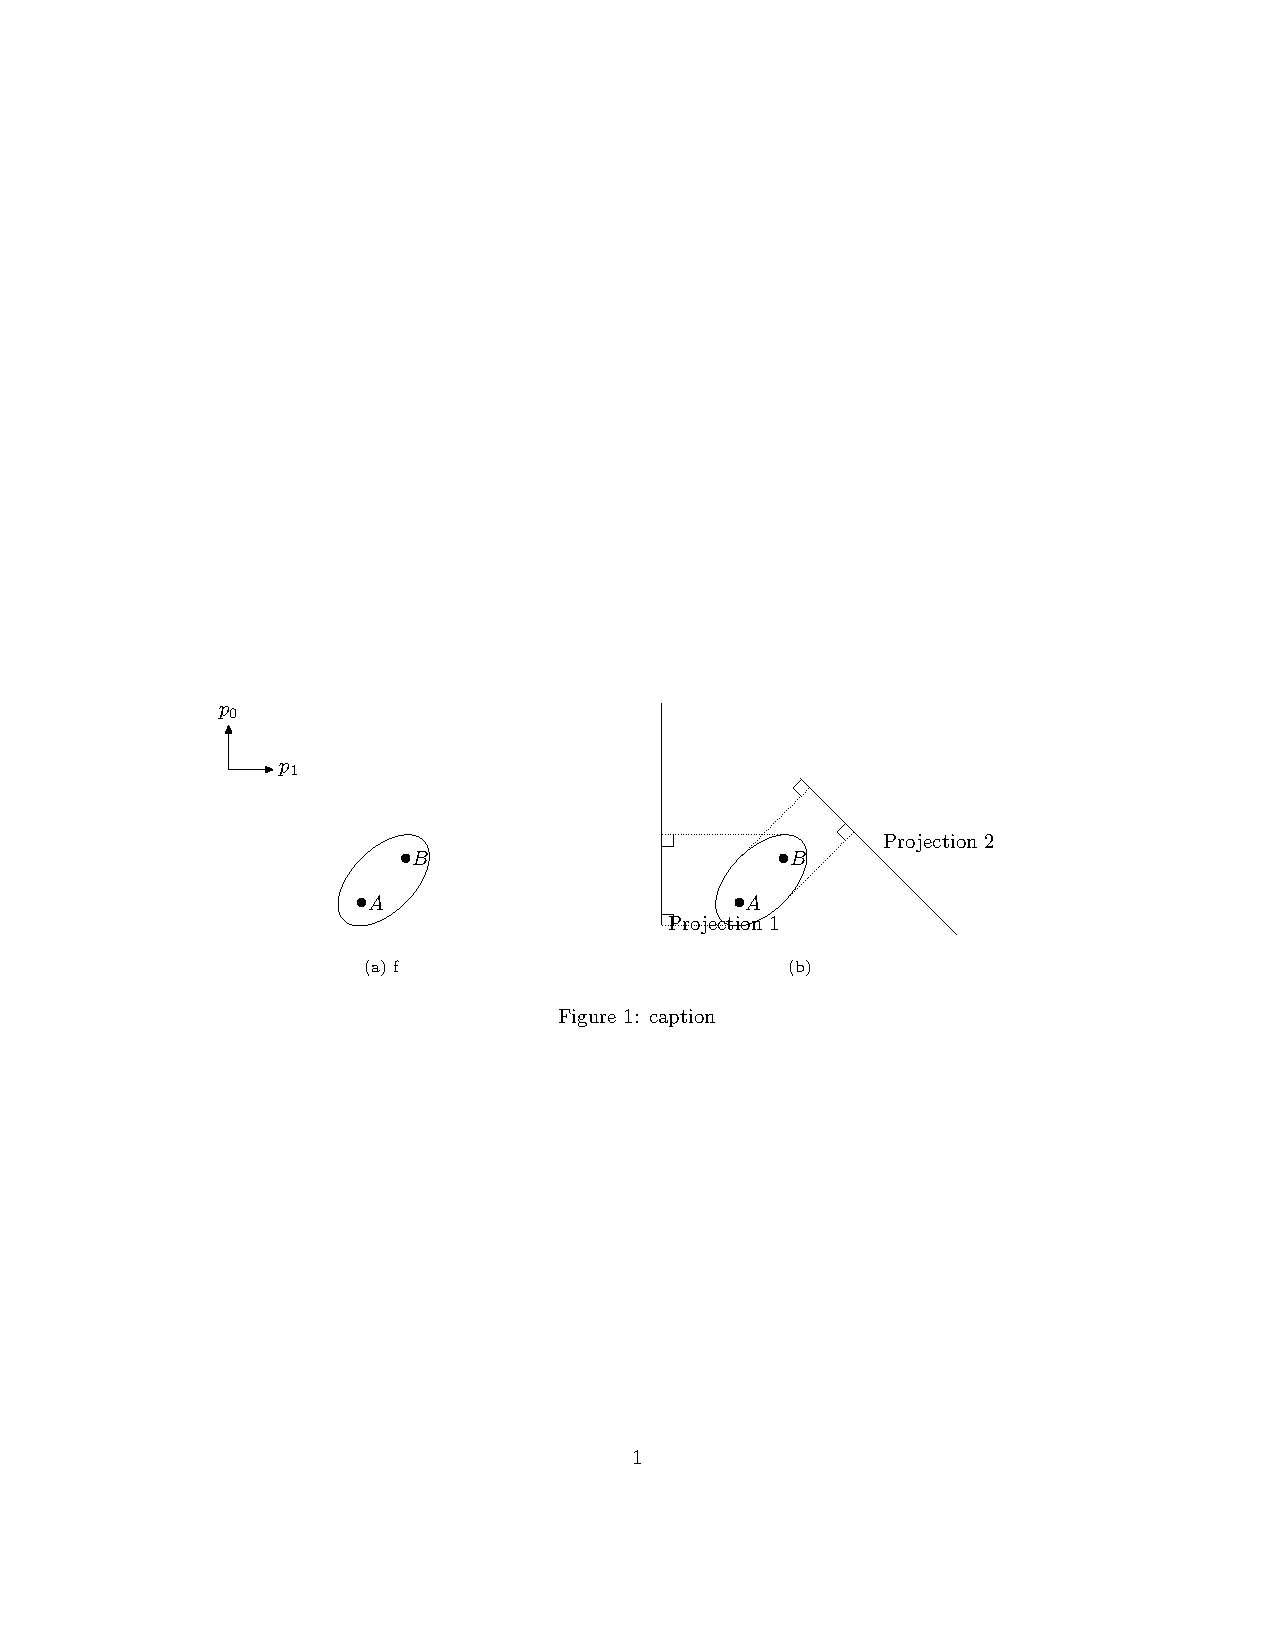
\includegraphics{measurement.8}}
%      \caption{caption}
%      \label{fig:Obs}
% \end{figure}

% \begin{figure}%[htp]
%      \centering
%      \subfigure[]{
%           \label{fig:ObsA}
%           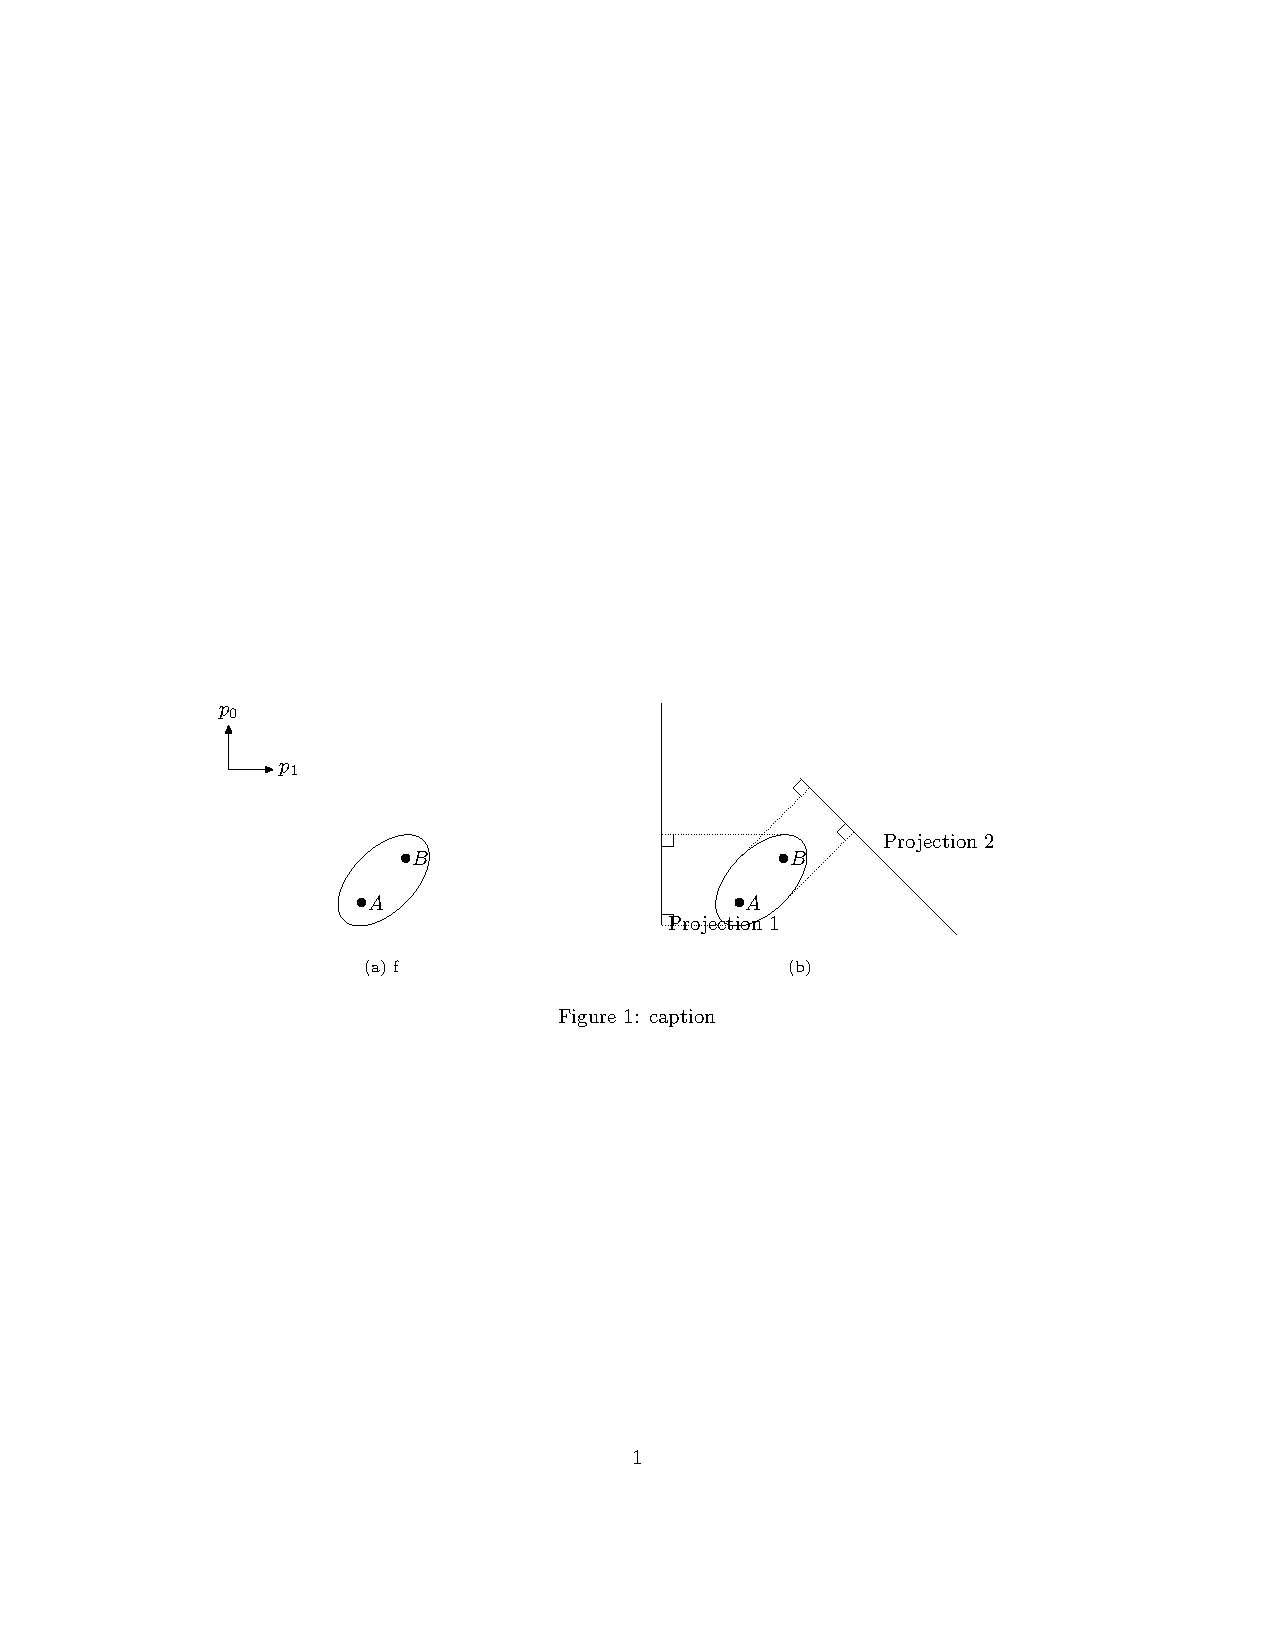
\includegraphics{measurement.9}}
%      \hspace{1cm}
%      \subfigure[]{
%           \label{fig:ObsB}
%           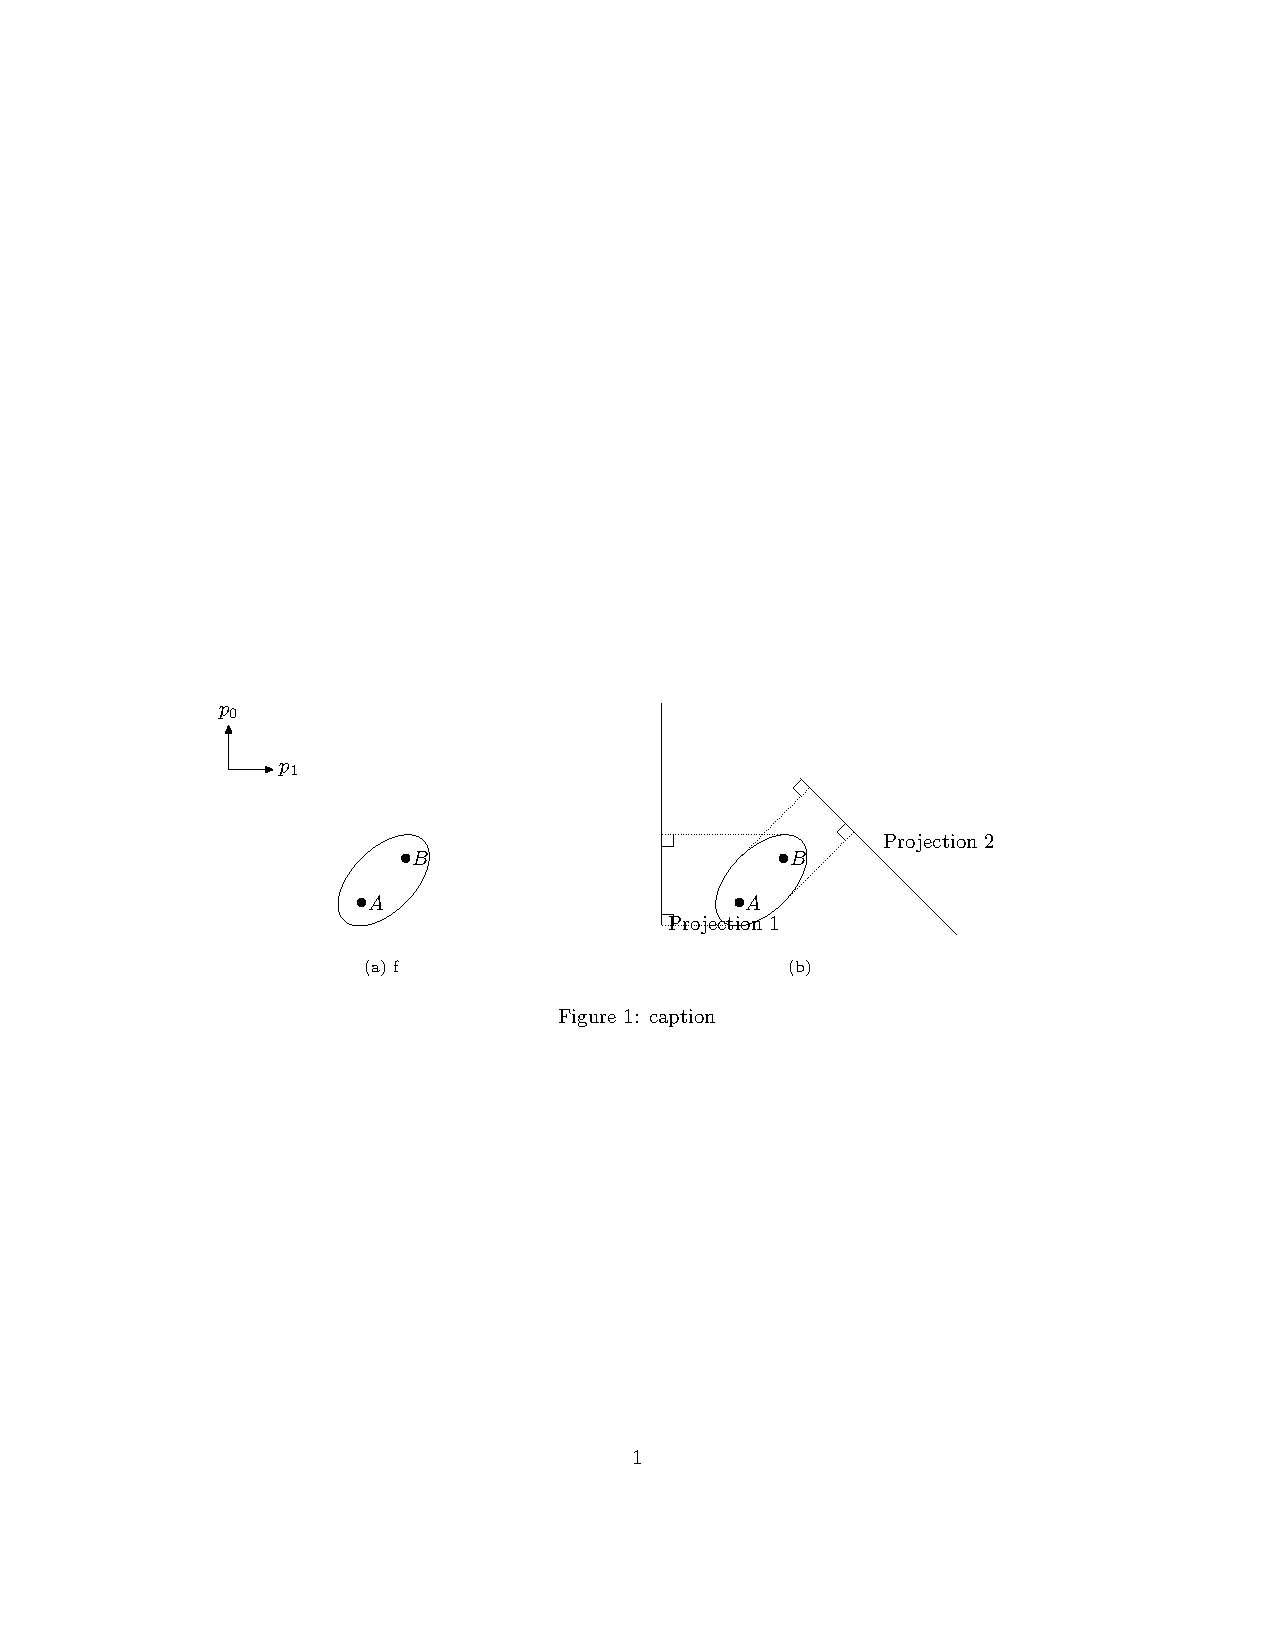
\includegraphics{measurement.10}}
%      \caption{caption}
%      \label{fig:Obs}
% \end{figure}

% %\includegraphics{lattice.3}
% %\includegraphics{lattice.4}
% %\includegraphics{lattice.5}

\end{document}
